\documentclass[]{elsarticle} %review=doublespace preprint=single 5p=2 column
%%% Begin My package additions %%%%%%%%%%%%%%%%%%%

\usepackage[hyphens]{url}

  \journal{Some Journal} % Sets Journal name

\usepackage{lineno} % add
  \linenumbers % turns line numbering on

\usepackage{graphicx}
%%%%%%%%%%%%%%%% end my additions to header

\usepackage[T1]{fontenc}
\usepackage{lmodern}
\usepackage{amssymb,amsmath}
\usepackage{ifxetex,ifluatex}
\usepackage{fixltx2e} % provides \textsubscript
% use upquote if available, for straight quotes in verbatim environments
\IfFileExists{upquote.sty}{\usepackage{upquote}}{}
\ifnum 0\ifxetex 1\fi\ifluatex 1\fi=0 % if pdftex
  \usepackage[utf8]{inputenc}
\else % if luatex or xelatex
  \usepackage{fontspec}
  \ifxetex
    \usepackage{xltxtra,xunicode}
  \fi
  \defaultfontfeatures{Mapping=tex-text,Scale=MatchLowercase}
  \newcommand{\euro}{€}
\fi
% use microtype if available
\IfFileExists{microtype.sty}{\usepackage{microtype}}{}
\usepackage[]{natbib}
\bibliographystyle{plainnat}

\ifxetex
  \usepackage[setpagesize=false, % page size defined by xetex
              unicode=false, % unicode breaks when used with xetex
              xetex]{hyperref}
\else
  \usepackage[unicode=true]{hyperref}
\fi
\hypersetup{breaklinks=true,
            bookmarks=true,
            pdfauthor={},
            pdftitle={Introducing spatial availability, a singly-constrained measure of competitive accessibility},
            colorlinks=false,
            urlcolor=blue,
            linkcolor=magenta,
            pdfborder={0 0 0}}

\setcounter{secnumdepth}{5}
% Pandoc toggle for numbering sections (defaults to be off)


% tightlist command for lists without linebreak
\providecommand{\tightlist}{%
  \setlength{\itemsep}{0pt}\setlength{\parskip}{0pt}}



\usepackage[font=small,skip=0pt]{caption}
\usepackage{booktabs}
\usepackage{longtable}
\usepackage{array}
\usepackage{multirow}
\usepackage{wrapfig}
\usepackage{float}
\usepackage{colortbl}
\usepackage{pdflscape}
\usepackage{tabu}
\usepackage{threeparttable}
\usepackage{threeparttablex}
\usepackage[normalem]{ulem}
\usepackage{makecell}
\usepackage{xcolor}
\usepackage{caption}
\usepackage{graphicx}
\usepackage{siunitx}
\usepackage{hhline}
\usepackage{calc}
\usepackage{tabularx}
\usepackage{adjustbox}
\usepackage{hyperref}



\begin{document}


\begin{frontmatter}

  \title{Introducing spatial availability, a singly-constrained measure
of competitive accessibility}
      \cortext[cor1]{Corresponding author}
  
  \begin{abstract}
  Accessibility indicators are widely used in transportation, urban, and
  healthcare planning, among many other applications. These measures are
  weighted sums of reachable opportunities from a given origin
  conditional on the cost of movement, and are estimates of the
  potential for spatial interaction. Over time, various proposals have
  been forwarded to improve their interpretability, mainly by
  introducing congestion and competition. In this paper we demonstrate
  how a widely used measure of accessibility with congestion fails to
  properly match the opportunity-seeking population. We then propose an
  alternative formulation of accessibility with competition, a measure
  we call \emph{spatial availability}. This measure results from using
  balancing factors that are equivalent to imposing a single constraint
  on conventional gravity-based accessibility. Further, we demonstrate
  how Two-Stage Floating Catchment Area methods can be seen as
  singly-constrained accessibility. To illustrate the application of
  spatial availability and compare it to other relevant measures, we use
  data from the 2016 Transportation Tomorrow Survey of the Greater
  Golden Horseshoe area in southern Ontario, Canada.
  \end{abstract}
  
 \end{frontmatter}

\newpage

\hypertarget{sec:introduction}{%
\section{Introduction}\label{sec:introduction}}

The concept of accessibility in transportation studies derives its
appeal from the combination of the spatial distribution of opportunities
and the cost of reaching them \citep{hansen1959, handy_measuring_1997}.
Accessibility analysis is employed in transportation, geography, public
health, and many other areas, with the number of applications growing
\citep{shi_literature_2020}, especially as mobility-based planning is
de-emphasized in favor of access-oriented planning
\citep{deboosere2018, handy2020, proffitt2017, yan2021}.

Numerous methods for calculating accessibility have been proposed in the
literature \citep{geurs2004}. Of these, gravity-type accessibility is
arguably the most common; since its introduction in the literature by
\citet{hansen1959}, it has been widely adopted in numerous forms
\citep{cervero_transportation_2002, paez2004network, geurs2004, levinson_accessibility_1998, Arranz2019measuring}.
Gravity-based accessibility indicators are essentially weighted sums of
opportunities, with the weights given by an impedance function that
depends on the cost of movement, and thus measure the \emph{intensity of
the possibility of interaction} \citep{hansen1959}. This type of
accessibility analysis offers a powerful tool to study the intersection
between urban structure and transportation infrastructure
\citep{handy_measuring_1997}.

Despite their utility, the interpretability of gravity-type
accessibility measures can be challenging \citep{geurs2004, miller2018}.
Since they aggregate opportunities, the results are sensitive to the
size of the region of interest (e.g., a large city has more jobs than a
smaller city). As a consequence, raw outputs are not necessarily
comparable across study areas \citep{allen2019}. This limitation becomes
evident when surveying studies that implement this type of analysis. For
example, \citet{paez_healthcare_2010} (in Montreal) and
\citet{campbell_2019_accessibility} (in Nairobi) report accessibility as
the number of health care facilities that can potentially be reached
from origins. But what does it mean for a zone to have accessibility to
less than 100 facilities in each of these two cities, with their
different populations and number of facilities? For that matter, what
does it mean for a zone to have accessibility to more than 700
facilities in Montreal, besides being ``accessibility rich''? As another
example, \citet{bocarejo_s_transport_2012} (in Bogota),
\citet{elgeneidy_cost_2016} (in Montreal), and
\citet{jiang_2016_accessibility} (in Beijing) report accessibility as
numbers of jobs, with accessibility values often in the hundreds of
thousands, and even exceeding one million jobs for some zones in Beijing
and Montreal. As indicators of urban structure, these measures are
informative, but the meaning of one million accessible jobs is harder to
pin down: how many jobs must any single person have access to? Clearly,
the answer to this question depends on how many people demand jobs.

The interpretability of gravity-type accessibility has been discussed in
numerous studies, including recently by \citet{hu_2019_measuring},
\citet{kelobonye2020measuring}, and in greater depth by
\citet{merlin2017competition}. As hinted above, the limitations in
interpretability are frequently caused by ignoring competition - without
competition, each opportunity is assumed to be equally available to
every single opportunity-seeking individual that can reach it
\citep{shen1998, paez2019, kelobonye2020measuring}. This assumption is
appropriate when the opportunity of interest is non-exclusive, that is,
if use by one unit of population does not preclude use by another. For
instance, national parks with abundant space are seldom used to full
capacity, so the presence of some population does not exclude use by
others. When it comes to exclusive opportunities, or when operations may
be affected by congestion, the solution has been to account for
competition. Several efforts exist that do so. In our reckoning, the
first such approach was proposed by \citet{weibull_axiomatic_1976},
whereby the distance decay of the supply of employment and the demand
for employment (by workers) were formulated under so-called axiomatic
assumptions. This approach was then applied by \citet{joseph1984} in the
context of healthcare, to quantify the availability of general
practitioners in Canada. About two decades later, \citet{shen1998}
independently re-discovered Weibull's
\citeyearpar{weibull_axiomatic_1976} formula \citep[see footnote (7)
in][]{shen1998} and deconstructed it to consider accessibility for
different modes. These advances were subsequently popularized as the
family of two-step floating catchment area (2SFCA) methods
\citep{luo2003} that have found widespread adoption in healthcare,
education, and food systems
\citep{yang_comparing_2006, chen_spatial_2020, ye_spatial_2018, chen_enhancing_2019, chen_evaluating_2020}.

An important development due to Shen was to show that the
population-weighted sum of the accessibility measure with competition
equates the number of opportunities available \citep[footnote (7) and
Appendix A in][]{shen1998}. This demonstration gave the impression of a
method that allocates all opportunities \emph{exactly}. In this paper we
intend to revisit accessibility with competition. We argue that Shen's
proof confuses the opportunity-seeking population with total zonal
population, an equivocation that results in misleading allocations of
opportunities to population that are masked by the presentation of
results as rates (i.e., opportunities per capita). We then propose an
alternative formulation of accessibility that incorporates competition
by adopting a proportional allocation mechanism. The use of balancing
factors for proportional allocation is akin to imposing a single
constraint on the accessibility indicator, in the spirit of Wilson's
\citeyearpar{wilson1971} spatial interaction model.

In this way, the aim of the paper is three-fold:

\begin{itemize}
\item
  First, we aim to demonstrate that Shen-type (and thus
  \citet{weibull_axiomatic_1976} accessibility and the popular 2SFCA
  methods) produce misleading estimates of the opportunities allocated;
\item
  Second, we introduce a new measure, \emph{spatial availability}, which
  we submit is a more interpretable alternative to Shen-style
  accessibility, since opportunities in the system are preserved and
  proportionally allocated to the population; and
\item
  Third, we show how Shen-type accessibility (and 2SFCA methods) can be
  seen as measures of singly-constrained accessibility.
\end{itemize}

Discussion is supported by the use of a small synthetic example drawn
from \citet{shen1998} and empirical data drawn from the 2016
Transportation Tomorrow Survey of the Greater Toronto and Hamilton Area
in Ontario, Canada. In the spirit of openness of research in the spatial
sciences \citep{brunsdon2021opening, paez2021open} this paper has a
companion open data product \citep{arribas2021Open}, and all code is
available for replicability and reproducibility purposes.

\hypertarget{background}{%
\section{Accesssibility measures revisited}\label{background}}

\hypertarget{hansen-type-accessibility}{%
\subsection{Hansen-type accessibility}\label{hansen-type-accessibility}}

Accessibility analysis stems from the foundational works of
\citet{harris_market_1954} and \citet{hansen1959}. From these seminal
efforts, many accessibility measures (excluding utility-based measures)
have been derived, particularly after the influential work of
\citet{wilson1971} on spatial interaction. The model follows the
formulation shown in Equation (\ref{eq:conventional-accessibility}):

\begin{equation}
\label{eq:conventional-accessibility}
S_i = \sum_{j=1}^JO_j \cdot f(c_{ij})
\end{equation}

\noindent where:

\begin{itemize}
\tightlist
\item
  \(S\) is Hansen-type accessibility.
\item
  \(i\) is a set of origin locations.
\item
  \(j\) is a set of destination locations.
\item
  \(O_j\) is the number of opportunities at location \(j\);
  \(\sum_j O_j\) is the total supply of opportunities in the study
  region.
\item
  \(c_{ij}\) is a measure of the cost of moving between \(i\) and \(j\).
\item
  \(f(\cdot)\) is an impedance function of \(c_{ij}\); it can take the
  form of any monotonically decreasing function chosen based on positive
  or normative criteria \citep{paez2012measuring}.
\end{itemize}

As formally defined, accessibility \(S_i\) is the sum of opportunities
that can be reached from location \(i\), weighted down by an impedance
function of the cost of travel \(c_{ij}\). Summing the opportunities in
the neighborhood of \(i\) provides estimates of the number of
opportunities that can \emph{potentially} be reached from \(i\). Several
variants of this method result from using a variety of impedance
functions; for example, cumulative opportunities measures are obtained
when \(f(\cdot)\) is a binary or indicator function
\citep[e.g.,][]{elgeneidy_cost_2016, rosik_forecast_2021, geurs2004, qi_decadelong_2018}.
Other measures use impedance functions modeled after any monotonically
decreasing function \citep[e.g., Gaussian, inverse power, negative
exponential, or log-normal, among others, see, \emph{inter
alia},][]{kwan_spacetime_1998, vale_influence_2017, reggiani_accessibility_2011, li_approach_2020}.
In practice, accessibility measures with different impedance functions
tend to be highly correlated
\citep{higgins2019, santanapalacios2022, kwan_spacetime_1998}.

Gravity-based accessibility has been shown to be an excellent indicator
of the intersection between urban structure and transportation
infrastructure
\citep{shi_literature_2020, reggiani_accessibility_2011, kwan_spacetime_1998}.
However, beyond enabling comparisons of relative values they are not
highly interpretable on their own \citep{miller2018}. To address the
issue or interpretability, previous research has aimed to index and
normalize values on a per demand-population basis
\citep[e.g.,][]{barboza_balancing_2021, pereira_distributional_2019, wang_access_2021}.
However, as recent research on accessibility discusses
\citep{merlin2017competition, allen2019, paez2019, kelobonye2020measuring},
these steps do not truly adequately consider competition. In effect,
when calculating \(S_i\), every opportunity enters the weighted sum once
for every origin \(i\) that can reach it. This makes interpretability
opaque, and to complicate matters, can also bias the estimated landscape
of opportunity.

\hypertarget{shen-type-competitive-accessibility}{%
\subsection{Shen-type competitive
accessibility}\label{shen-type-competitive-accessibility}}

To account for competition, the influential works of \citet{shen1998}
and \citet{weibull_axiomatic_1976}, as well as the widely used 2SFCA
approach of \citet{luo2003}, adjust Hansen-type accessibility with the
population in the region of interest. The mechanics of this approach
consist of calculating, for every destination \(j\), the population that
can reach it given the impedance function \(f(\cdot)\). \citet{shen1998}
calls this ``the opportunity-seeking population''. The opportunities at
\(j\) are then divided by their corresponding opportunity-seeking
population to obtain a measure of opportunities per capita, i.e.,
\(R_j\) in Equation (\ref{eq:2SFCA-step1}). Per capita values are then
allocated back to the population at \(i\), again subject to the
impedance function. Equation (\ref{eq:2SFCA-step1}) corresponds to the
first step of this procedure, and Equation (\ref{eq:2SFCA-step2}) to the
second.

\begin{equation}
\label{eq:2SFCA-step1}
R_{j} = \frac{O_{j}}{\sum_i P_{i} \cdot f(c_{ij})}\\
\end{equation}

\begin{equation}
\label{eq:2SFCA-step2}
A_{i} = {\sum_j R_{j} \cdot f(c_{ij})}\\
\end{equation}

\noindent where:

\begin{itemize}
\tightlist
\item
  \(A\) is Shen-type accessibility.
\item
  \(i\) is a set of origin locations.
\item
  \(j\) is a set of destination locations.
\item
  \(O_j\) is the number of opportunities at location \(j\);
\item
  \(P_i\) is the population at location \(i\); \(\sum_j R_j\) is the
  total supply of opportunities in the study region.
\item
  \(R_j\) is the provider-to-population (PPR) ratio at location \(j\);
\item
  \(c_{ij}\) is a measure of the cost of moving between \(i\) and \(j\);
\item
  \(f(\cdot)\) is an impedance function of \(c_{ij}\).
\end{itemize}

As noted above, \citet{shen1998} furnished a demonstration that the
resulting values of \(A_i\), when multiplied by the population at that
origin and summed for the full study region, equates the total number of
opportunities in the full study region. But is this really the case?

\hypertarget{example}{%
\subsection{Example}\label{example}}

To motivate the discussion, we begin with the example in
\citet{shen1998}. This is the simple system shown in Figure
\ref{fig:plot-toy-example}.

\begin{figure}

{\centering 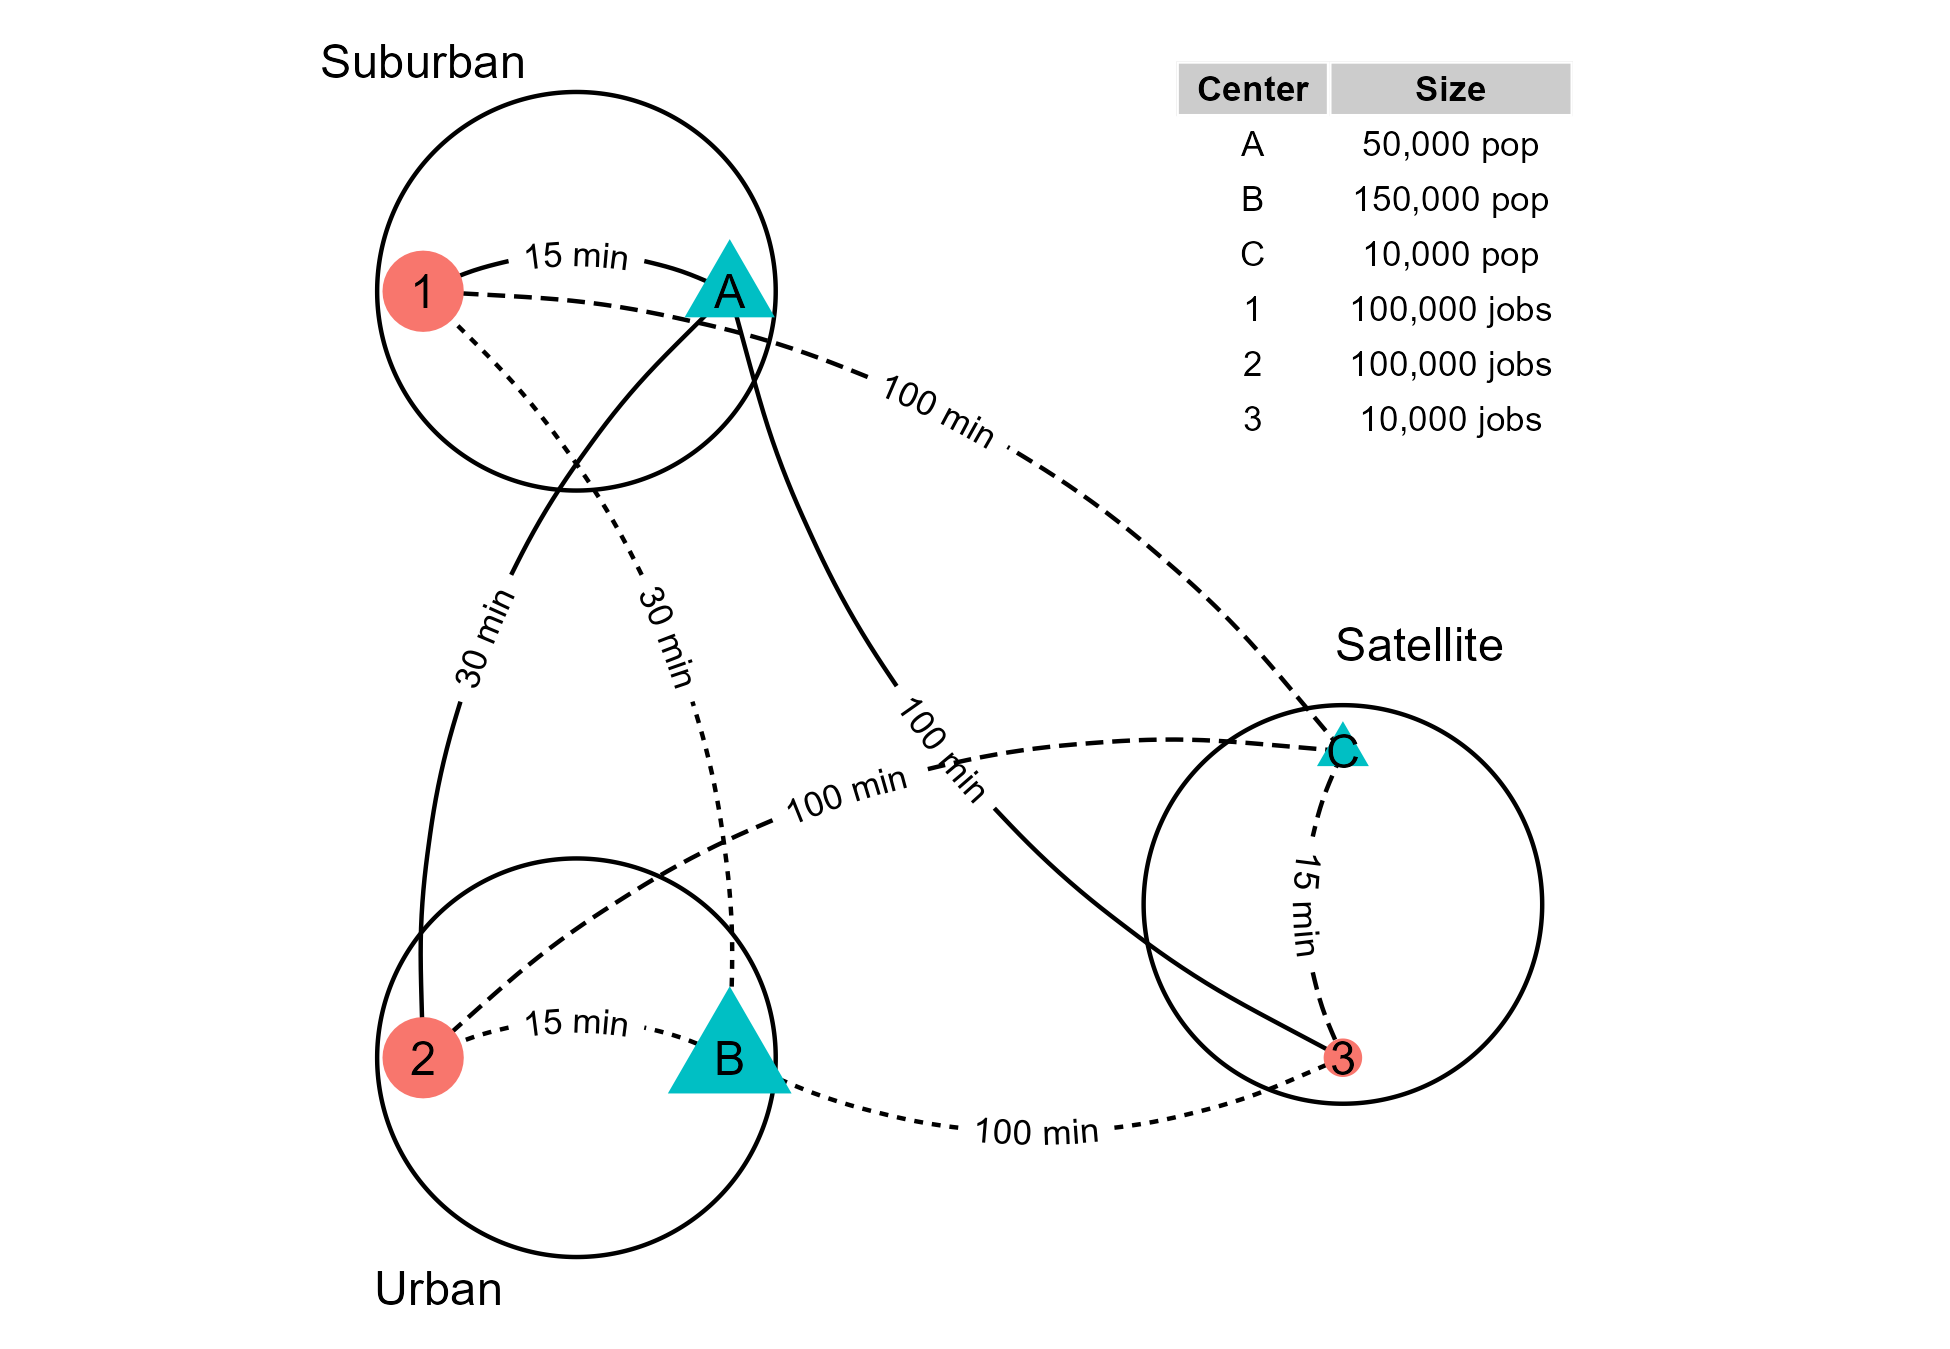
\includegraphics[width=1\linewidth]{images/plot-toy-example} 

}

\caption{\label{fig:plot-toy-example} Shen (1998) synthetic example with locations of employment centers (in orange), population centers (in blue), number of jobs and population, and travel times.}\label{fig:create-figure-with-toy-example3}
\end{figure}

 
  \providecommand{\huxb}[2]{\arrayrulecolor[RGB]{#1}\global\arrayrulewidth=#2pt}
  \providecommand{\huxvb}[2]{\color[RGB]{#1}\vrule width #2pt}
  \providecommand{\huxtpad}[1]{\rule{0pt}{#1}}
  \providecommand{\huxbpad}[1]{\rule[-#1]{0pt}{#1}}

\begin{table}[ht]
\begin{centerbox}
\begin{threeparttable}
\captionsetup{justification=centering,singlelinecheck=off}
\caption{Summary description of synthetic example: Hansen-type accessibility and Shen-type accessibility with competition}
 \label{tab:synthetic-example}
\setlength{\tabcolsep}{0pt}
\begin{tabularx}{1.2\textwidth}{p{0.12\textwidth} p{0.12\textwidth} p{0.12\textwidth} p{0.12\textwidth} p{0.12\textwidth} p{0.12\textwidth} p{0.12\textwidth} p{0.12\textwidth} p{0.12\textwidth} p{0.12\textwidth}}


\hhline{>{\huxb{190, 190, 190}{1}}|>{\huxb{190, 190, 190}{1}}|>{\huxb{190, 190, 190}{1}}|>{\huxb{190, 190, 190}{1}}|>{\huxb{190, 190, 190}{1}}|>{\huxb{190, 190, 190}{1}}|>{\huxb{190, 190, 190}{1}}|>{\huxb{190, 190, 190}{1}}|>{\huxb{190, 190, 190}{1}}|}
\arrayrulecolor{black}

\multicolumn{1}{!{\huxvb{0, 0, 0}{0}}p{0.12\textwidth}!{\huxvb{190, 190, 190}{1}}}{\hspace{6pt}\parbox[b]{0.12\textwidth-6pt-6pt}{\huxtpad{6pt + 1em}\raggedright \textbf{{\fontsize{7pt}{8.4pt}\selectfont Origin}}\huxbpad{6pt}}} &
\multicolumn{1}{p{0.12\textwidth}!{\huxvb{190, 190, 190}{1}}}{\hspace{6pt}\parbox[b]{0.12\textwidth-6pt-6pt}{\huxtpad{6pt + 1em}\centering \textbf{{\fontsize{7pt}{8.4pt}\selectfont Pop.}}\huxbpad{6pt}}} &
\multicolumn{1}{p{0.12\textwidth}!{\huxvb{190, 190, 190}{1}}}{\hspace{6pt}\parbox[b]{0.12\textwidth-6pt-6pt}{\huxtpad{6pt + 1em}\raggedright \textbf{{\fontsize{7pt}{8.4pt}\selectfont Dest.}}\huxbpad{6pt}}} &
\multicolumn{1}{p{0.12\textwidth}!{\huxvb{190, 190, 190}{1}}}{\hspace{6pt}\parbox[b]{0.12\textwidth-6pt-6pt}{\huxtpad{6pt + 1em}\centering \textbf{{\fontsize{7pt}{8.4pt}\selectfont Jobs}}\huxbpad{6pt}}} &
\multicolumn{1}{p{0.12\textwidth}!{\huxvb{190, 190, 190}{1}}}{\hspace{6pt}\parbox[b]{0.12\textwidth-6pt-6pt}{\huxtpad{6pt + 1em}\centering \textbf{{\fontsize{7pt}{8.4pt}\selectfont TT}}\huxbpad{6pt}}} &
\multicolumn{1}{p{0.12\textwidth}!{\huxvb{190, 190, 190}{1}}}{\hspace{6pt}\parbox[b]{0.12\textwidth-6pt-6pt}{\huxtpad{6pt + 1em}\centering \textbf{{\fontsize{7pt}{8.4pt}\selectfont f(TT)}}\huxbpad{6pt}}} &
\multicolumn{1}{p{0.12\textwidth}!{\huxvb{190, 190, 190}{1}}}{\hspace{6pt}\parbox[b]{0.12\textwidth-6pt-6pt}{\huxtpad{6pt + 1em}\centering \textbf{{\fontsize{7pt}{8.4pt}\selectfont Pop * f(TT)}}\huxbpad{6pt}}} &
\multicolumn{1}{p{0.12\textwidth}!{\huxvb{190, 190, 190}{1}}}{\hspace{6pt}\parbox[b]{0.12\textwidth-6pt-6pt}{\huxtpad{6pt + 1em}\centering \textbf{{\fontsize{7pt}{8.4pt}\selectfont Jobs * f(TT)}}\huxbpad{6pt}}} &
\multicolumn{1}{p{0.12\textwidth}!{\huxvb{190, 190, 190}{1}}}{\hspace{6pt}\parbox[b]{0.12\textwidth-6pt-6pt}{\huxtpad{6pt + 1em}\centering \textbf{{\fontsize{7pt}{8.4pt}\selectfont S\_i}}\huxbpad{6pt}}} &
\multicolumn{1}{p{0.12\textwidth}!{\huxvb{0, 0, 0}{0}}}{\hspace{6pt}\parbox[b]{0.12\textwidth-6pt-6pt}{\huxtpad{6pt + 1em}\centering \textbf{{\fontsize{7pt}{8.4pt}\selectfont A\_i}}\huxbpad{6pt}}} \tabularnewline[-0.5pt]


\hhline{>{\huxb{0, 0, 0}{0.4}}->{\huxb{0, 0, 0}{0.4}}->{\huxb{0, 0, 0}{0.4}}->{\huxb{0, 0, 0}{0.4}}->{\huxb{0, 0, 0}{0.4}}->{\huxb{0, 0, 0}{0.4}}->{\huxb{0, 0, 0}{0.4}}->{\huxb{0, 0, 0}{0.4}}->{\huxb{0, 0, 0}{0.4}}->{\huxb{0, 0, 0}{0.4}}-}
\arrayrulecolor{black}

\multicolumn{1}{!{\huxvb{0, 0, 0}{0}}p{0.12\textwidth}!{\huxvb{190, 190, 190}{1}}}{} &
\multicolumn{1}{p{0.12\textwidth}!{\huxvb{190, 190, 190}{1}}}{} &
\multicolumn{1}{p{0.12\textwidth}!{\huxvb{190, 190, 190}{1}}}{\hspace{6pt}\parbox[b]{0.12\textwidth-6pt-6pt}{\huxtpad{6pt + 1em}\raggedright {\fontsize{7pt}{8.4pt}\selectfont 1}\huxbpad{6pt}}} &
\multicolumn{1}{p{0.12\textwidth}!{\huxvb{190, 190, 190}{1}}}{\hspace{6pt}\parbox[b]{0.12\textwidth-6pt-6pt}{\huxtpad{6pt + 1em}\centering {\fontsize{7pt}{8.4pt}\selectfont 100,000}\huxbpad{6pt}}} &
\multicolumn{1}{p{0.12\textwidth}!{\huxvb{190, 190, 190}{1}}}{\hspace{6pt}\parbox[b]{0.12\textwidth-6pt-6pt}{\huxtpad{6pt + 1em}\centering {\fontsize{7pt}{8.4pt}\selectfont 15}\huxbpad{6pt}}} &
\multicolumn{1}{p{0.12\textwidth}!{\huxvb{190, 190, 190}{1}}}{\hspace{6pt}\parbox[b]{0.12\textwidth-6pt-6pt}{\huxtpad{6pt + 1em}\centering {\fontsize{7pt}{8.4pt}\selectfont 0.223130}\huxbpad{6pt}}} &
\multicolumn{1}{p{0.12\textwidth}!{\huxvb{190, 190, 190}{1}}}{\hspace{6pt}\parbox[b]{0.12\textwidth-6pt-6pt}{\huxtpad{6pt + 1em}\centering {\fontsize{7pt}{8.4pt}\selectfont 11,157}\huxbpad{6pt}}} &
\multicolumn{1}{p{0.12\textwidth}!{\huxvb{190, 190, 190}{1}}}{\hspace{6pt}\parbox[b]{0.12\textwidth-6pt-6pt}{\huxtpad{6pt + 1em}\centering {\fontsize{7pt}{8.4pt}\selectfont 22,313}\huxbpad{6pt}}} &
\multicolumn{1}{p{0.12\textwidth}!{\huxvb{190, 190, 190}{1}}}{} &
\multicolumn{1}{p{0.12\textwidth}!{\huxvb{0, 0, 0}{0}}}{} \tabularnewline[-0.5pt]


\hhline{>{\huxb{190, 190, 190}{1}}|>{\huxb{190, 190, 190}{1}}|>{\huxb{190, 190, 190}{1}}|>{\huxb{190, 190, 190}{1}}|>{\huxb{190, 190, 190}{1}}|>{\huxb{190, 190, 190}{1}}|>{\huxb{190, 190, 190}{1}}|>{\huxb{190, 190, 190}{1}}|>{\huxb{190, 190, 190}{1}}|}
\arrayrulecolor{black}

\multicolumn{1}{!{\huxvb{0, 0, 0}{0}}p{0.12\textwidth}!{\huxvb{190, 190, 190}{1}}}{} &
\multicolumn{1}{p{0.12\textwidth}!{\huxvb{190, 190, 190}{1}}}{} &
\multicolumn{1}{p{0.12\textwidth}!{\huxvb{190, 190, 190}{1}}}{\hspace{6pt}\parbox[b]{0.12\textwidth-6pt-6pt}{\huxtpad{6pt + 1em}\raggedright {\fontsize{7pt}{8.4pt}\selectfont 2}\huxbpad{6pt}}} &
\multicolumn{1}{p{0.12\textwidth}!{\huxvb{190, 190, 190}{1}}}{\hspace{6pt}\parbox[b]{0.12\textwidth-6pt-6pt}{\huxtpad{6pt + 1em}\centering {\fontsize{7pt}{8.4pt}\selectfont 100,000}\huxbpad{6pt}}} &
\multicolumn{1}{p{0.12\textwidth}!{\huxvb{190, 190, 190}{1}}}{\hspace{6pt}\parbox[b]{0.12\textwidth-6pt-6pt}{\huxtpad{6pt + 1em}\centering {\fontsize{7pt}{8.4pt}\selectfont 30}\huxbpad{6pt}}} &
\multicolumn{1}{p{0.12\textwidth}!{\huxvb{190, 190, 190}{1}}}{\hspace{6pt}\parbox[b]{0.12\textwidth-6pt-6pt}{\huxtpad{6pt + 1em}\centering {\fontsize{7pt}{8.4pt}\selectfont 0.049787}\huxbpad{6pt}}} &
\multicolumn{1}{p{0.12\textwidth}!{\huxvb{190, 190, 190}{1}}}{\hspace{6pt}\parbox[b]{0.12\textwidth-6pt-6pt}{\huxtpad{6pt + 1em}\centering {\fontsize{7pt}{8.4pt}\selectfont 2,489}\huxbpad{6pt}}} &
\multicolumn{1}{p{0.12\textwidth}!{\huxvb{190, 190, 190}{1}}}{\hspace{6pt}\parbox[b]{0.12\textwidth-6pt-6pt}{\huxtpad{6pt + 1em}\centering {\fontsize{7pt}{8.4pt}\selectfont 4,979}\huxbpad{6pt}}} &
\multicolumn{1}{p{0.12\textwidth}!{\huxvb{190, 190, 190}{1}}}{} &
\multicolumn{1}{p{0.12\textwidth}!{\huxvb{0, 0, 0}{0}}}{} \tabularnewline[-0.5pt]


\hhline{>{\huxb{190, 190, 190}{1}}|>{\huxb{190, 190, 190}{1}}|>{\huxb{190, 190, 190}{1}}|>{\huxb{190, 190, 190}{1}}|>{\huxb{190, 190, 190}{1}}|>{\huxb{190, 190, 190}{1}}|>{\huxb{190, 190, 190}{1}}|>{\huxb{190, 190, 190}{1}}|>{\huxb{190, 190, 190}{1}}|}
\arrayrulecolor{black}

\multicolumn{1}{!{\huxvb{0, 0, 0}{0}}p{0.12\textwidth}!{\huxvb{190, 190, 190}{1}}}{\multirow[t]{-3}{*}[0ex]{\hspace{6pt}\parbox[b]{0.12\textwidth-6pt-6pt}{\huxtpad{6pt + 1em}\raggedright {\fontsize{7pt}{8.4pt}\selectfont A}\huxbpad{6pt}}}} &
\multicolumn{1}{p{0.12\textwidth}!{\huxvb{190, 190, 190}{1}}}{\multirow[t]{-3}{*}[0ex]{\hspace{6pt}\parbox[b]{0.12\textwidth-6pt-6pt}{\huxtpad{6pt + 1em}\centering {\fontsize{7pt}{8.4pt}\selectfont 50,000}\huxbpad{6pt}}}} &
\multicolumn{1}{p{0.12\textwidth}!{\huxvb{190, 190, 190}{1}}}{\hspace{6pt}\parbox[b]{0.12\textwidth-6pt-6pt}{\huxtpad{6pt + 1em}\raggedright {\fontsize{7pt}{8.4pt}\selectfont 3}\huxbpad{6pt}}} &
\multicolumn{1}{p{0.12\textwidth}!{\huxvb{190, 190, 190}{1}}}{\hspace{6pt}\parbox[b]{0.12\textwidth-6pt-6pt}{\huxtpad{6pt + 1em}\centering {\fontsize{7pt}{8.4pt}\selectfont 10,000}\huxbpad{6pt}}} &
\multicolumn{1}{p{0.12\textwidth}!{\huxvb{190, 190, 190}{1}}}{\hspace{6pt}\parbox[b]{0.12\textwidth-6pt-6pt}{\huxtpad{6pt + 1em}\centering {\fontsize{7pt}{8.4pt}\selectfont 100}\huxbpad{6pt}}} &
\multicolumn{1}{p{0.12\textwidth}!{\huxvb{190, 190, 190}{1}}}{\hspace{6pt}\parbox[b]{0.12\textwidth-6pt-6pt}{\huxtpad{6pt + 1em}\centering {\fontsize{7pt}{8.4pt}\selectfont 0.000045}\huxbpad{6pt}}} &
\multicolumn{1}{p{0.12\textwidth}!{\huxvb{190, 190, 190}{1}}}{\hspace{6pt}\parbox[b]{0.12\textwidth-6pt-6pt}{\huxtpad{6pt + 1em}\centering {\fontsize{7pt}{8.4pt}\selectfont 2.27}\huxbpad{6pt}}} &
\multicolumn{1}{p{0.12\textwidth}!{\huxvb{190, 190, 190}{1}}}{\hspace{6pt}\parbox[b]{0.12\textwidth-6pt-6pt}{\huxtpad{6pt + 1em}\centering {\fontsize{7pt}{8.4pt}\selectfont 0.454}\huxbpad{6pt}}} &
\multicolumn{1}{p{0.12\textwidth}!{\huxvb{190, 190, 190}{1}}}{\multirow[t]{-3}{*}[0ex]{\hspace{6pt}\parbox[b]{0.12\textwidth-6pt-6pt}{\huxtpad{6pt + 1em}\centering {\fontsize{7pt}{8.4pt}\selectfont 27,292}\huxbpad{6pt}}}} &
\multicolumn{1}{p{0.12\textwidth}!{\huxvb{0, 0, 0}{0}}}{\multirow[t]{-3}{*}[0ex]{\hspace{6pt}\parbox[b]{0.12\textwidth-6pt-6pt}{\huxtpad{6pt + 1em}\centering {\fontsize{7pt}{8.4pt}\selectfont 1.34}\huxbpad{6pt}}}} \tabularnewline[-0.5pt]


\hhline{>{\huxb{0, 0, 0}{0.4}}->{\huxb{0, 0, 0}{0.4}}->{\huxb{0, 0, 0}{0.4}}->{\huxb{0, 0, 0}{0.4}}->{\huxb{0, 0, 0}{0.4}}->{\huxb{0, 0, 0}{0.4}}->{\huxb{0, 0, 0}{0.4}}->{\huxb{0, 0, 0}{0.4}}->{\huxb{0, 0, 0}{0.4}}->{\huxb{0, 0, 0}{0.4}}-}
\arrayrulecolor{black}

\multicolumn{1}{!{\huxvb{0, 0, 0}{0}}p{0.12\textwidth}!{\huxvb{190, 190, 190}{1}}}{} &
\multicolumn{1}{p{0.12\textwidth}!{\huxvb{190, 190, 190}{1}}}{} &
\multicolumn{1}{p{0.12\textwidth}!{\huxvb{190, 190, 190}{1}}}{\hspace{6pt}\parbox[b]{0.12\textwidth-6pt-6pt}{\huxtpad{6pt + 1em}\raggedright {\fontsize{7pt}{8.4pt}\selectfont 1}\huxbpad{6pt}}} &
\multicolumn{1}{p{0.12\textwidth}!{\huxvb{190, 190, 190}{1}}}{\hspace{6pt}\parbox[b]{0.12\textwidth-6pt-6pt}{\huxtpad{6pt + 1em}\centering {\fontsize{7pt}{8.4pt}\selectfont 100,000}\huxbpad{6pt}}} &
\multicolumn{1}{p{0.12\textwidth}!{\huxvb{190, 190, 190}{1}}}{\hspace{6pt}\parbox[b]{0.12\textwidth-6pt-6pt}{\huxtpad{6pt + 1em}\centering {\fontsize{7pt}{8.4pt}\selectfont 30}\huxbpad{6pt}}} &
\multicolumn{1}{p{0.12\textwidth}!{\huxvb{190, 190, 190}{1}}}{\hspace{6pt}\parbox[b]{0.12\textwidth-6pt-6pt}{\huxtpad{6pt + 1em}\centering {\fontsize{7pt}{8.4pt}\selectfont 0.049787}\huxbpad{6pt}}} &
\multicolumn{1}{p{0.12\textwidth}!{\huxvb{190, 190, 190}{1}}}{\hspace{6pt}\parbox[b]{0.12\textwidth-6pt-6pt}{\huxtpad{6pt + 1em}\centering {\fontsize{7pt}{8.4pt}\selectfont 7,468}\huxbpad{6pt}}} &
\multicolumn{1}{p{0.12\textwidth}!{\huxvb{190, 190, 190}{1}}}{\hspace{6pt}\parbox[b]{0.12\textwidth-6pt-6pt}{\huxtpad{6pt + 1em}\centering {\fontsize{7pt}{8.4pt}\selectfont 4,979}\huxbpad{6pt}}} &
\multicolumn{1}{p{0.12\textwidth}!{\huxvb{190, 190, 190}{1}}}{} &
\multicolumn{1}{p{0.12\textwidth}!{\huxvb{0, 0, 0}{0}}}{} \tabularnewline[-0.5pt]


\hhline{>{\huxb{190, 190, 190}{1}}|>{\huxb{190, 190, 190}{1}}|>{\huxb{190, 190, 190}{1}}|>{\huxb{190, 190, 190}{1}}|>{\huxb{190, 190, 190}{1}}|>{\huxb{190, 190, 190}{1}}|>{\huxb{190, 190, 190}{1}}|>{\huxb{190, 190, 190}{1}}|>{\huxb{190, 190, 190}{1}}|}
\arrayrulecolor{black}

\multicolumn{1}{!{\huxvb{0, 0, 0}{0}}p{0.12\textwidth}!{\huxvb{190, 190, 190}{1}}}{} &
\multicolumn{1}{p{0.12\textwidth}!{\huxvb{190, 190, 190}{1}}}{} &
\multicolumn{1}{p{0.12\textwidth}!{\huxvb{190, 190, 190}{1}}}{\hspace{6pt}\parbox[b]{0.12\textwidth-6pt-6pt}{\huxtpad{6pt + 1em}\raggedright {\fontsize{7pt}{8.4pt}\selectfont 2}\huxbpad{6pt}}} &
\multicolumn{1}{p{0.12\textwidth}!{\huxvb{190, 190, 190}{1}}}{\hspace{6pt}\parbox[b]{0.12\textwidth-6pt-6pt}{\huxtpad{6pt + 1em}\centering {\fontsize{7pt}{8.4pt}\selectfont 100,000}\huxbpad{6pt}}} &
\multicolumn{1}{p{0.12\textwidth}!{\huxvb{190, 190, 190}{1}}}{\hspace{6pt}\parbox[b]{0.12\textwidth-6pt-6pt}{\huxtpad{6pt + 1em}\centering {\fontsize{7pt}{8.4pt}\selectfont 15}\huxbpad{6pt}}} &
\multicolumn{1}{p{0.12\textwidth}!{\huxvb{190, 190, 190}{1}}}{\hspace{6pt}\parbox[b]{0.12\textwidth-6pt-6pt}{\huxtpad{6pt + 1em}\centering {\fontsize{7pt}{8.4pt}\selectfont 0.223130}\huxbpad{6pt}}} &
\multicolumn{1}{p{0.12\textwidth}!{\huxvb{190, 190, 190}{1}}}{\hspace{6pt}\parbox[b]{0.12\textwidth-6pt-6pt}{\huxtpad{6pt + 1em}\centering {\fontsize{7pt}{8.4pt}\selectfont 33,470}\huxbpad{6pt}}} &
\multicolumn{1}{p{0.12\textwidth}!{\huxvb{190, 190, 190}{1}}}{\hspace{6pt}\parbox[b]{0.12\textwidth-6pt-6pt}{\huxtpad{6pt + 1em}\centering {\fontsize{7pt}{8.4pt}\selectfont 22,313}\huxbpad{6pt}}} &
\multicolumn{1}{p{0.12\textwidth}!{\huxvb{190, 190, 190}{1}}}{} &
\multicolumn{1}{p{0.12\textwidth}!{\huxvb{0, 0, 0}{0}}}{} \tabularnewline[-0.5pt]


\hhline{>{\huxb{190, 190, 190}{1}}|>{\huxb{190, 190, 190}{1}}|>{\huxb{190, 190, 190}{1}}|>{\huxb{190, 190, 190}{1}}|>{\huxb{190, 190, 190}{1}}|>{\huxb{190, 190, 190}{1}}|>{\huxb{190, 190, 190}{1}}|>{\huxb{190, 190, 190}{1}}|>{\huxb{190, 190, 190}{1}}|}
\arrayrulecolor{black}

\multicolumn{1}{!{\huxvb{0, 0, 0}{0}}p{0.12\textwidth}!{\huxvb{190, 190, 190}{1}}}{\multirow[t]{-3}{*}[0ex]{\hspace{6pt}\parbox[b]{0.12\textwidth-6pt-6pt}{\huxtpad{6pt + 1em}\raggedright {\fontsize{7pt}{8.4pt}\selectfont B}\huxbpad{6pt}}}} &
\multicolumn{1}{p{0.12\textwidth}!{\huxvb{190, 190, 190}{1}}}{\multirow[t]{-3}{*}[0ex]{\hspace{6pt}\parbox[b]{0.12\textwidth-6pt-6pt}{\huxtpad{6pt + 1em}\centering {\fontsize{7pt}{8.4pt}\selectfont 150,000}\huxbpad{6pt}}}} &
\multicolumn{1}{p{0.12\textwidth}!{\huxvb{190, 190, 190}{1}}}{\hspace{6pt}\parbox[b]{0.12\textwidth-6pt-6pt}{\huxtpad{6pt + 1em}\raggedright {\fontsize{7pt}{8.4pt}\selectfont 3}\huxbpad{6pt}}} &
\multicolumn{1}{p{0.12\textwidth}!{\huxvb{190, 190, 190}{1}}}{\hspace{6pt}\parbox[b]{0.12\textwidth-6pt-6pt}{\huxtpad{6pt + 1em}\centering {\fontsize{7pt}{8.4pt}\selectfont 10,000}\huxbpad{6pt}}} &
\multicolumn{1}{p{0.12\textwidth}!{\huxvb{190, 190, 190}{1}}}{\hspace{6pt}\parbox[b]{0.12\textwidth-6pt-6pt}{\huxtpad{6pt + 1em}\centering {\fontsize{7pt}{8.4pt}\selectfont 100}\huxbpad{6pt}}} &
\multicolumn{1}{p{0.12\textwidth}!{\huxvb{190, 190, 190}{1}}}{\hspace{6pt}\parbox[b]{0.12\textwidth-6pt-6pt}{\huxtpad{6pt + 1em}\centering {\fontsize{7pt}{8.4pt}\selectfont 0.000045}\huxbpad{6pt}}} &
\multicolumn{1}{p{0.12\textwidth}!{\huxvb{190, 190, 190}{1}}}{\hspace{6pt}\parbox[b]{0.12\textwidth-6pt-6pt}{\huxtpad{6pt + 1em}\centering {\fontsize{7pt}{8.4pt}\selectfont 6.81}\huxbpad{6pt}}} &
\multicolumn{1}{p{0.12\textwidth}!{\huxvb{190, 190, 190}{1}}}{\hspace{6pt}\parbox[b]{0.12\textwidth-6pt-6pt}{\huxtpad{6pt + 1em}\centering {\fontsize{7pt}{8.4pt}\selectfont 0.454}\huxbpad{6pt}}} &
\multicolumn{1}{p{0.12\textwidth}!{\huxvb{190, 190, 190}{1}}}{\multirow[t]{-3}{*}[0ex]{\hspace{6pt}\parbox[b]{0.12\textwidth-6pt-6pt}{\huxtpad{6pt + 1em}\centering {\fontsize{7pt}{8.4pt}\selectfont 27,292}\huxbpad{6pt}}}} &
\multicolumn{1}{p{0.12\textwidth}!{\huxvb{0, 0, 0}{0}}}{\multirow[t]{-3}{*}[0ex]{\hspace{6pt}\parbox[b]{0.12\textwidth-6pt-6pt}{\huxtpad{6pt + 1em}\centering {\fontsize{7pt}{8.4pt}\selectfont 0.888}\huxbpad{6pt}}}} \tabularnewline[-0.5pt]


\hhline{>{\huxb{0, 0, 0}{0.4}}->{\huxb{0, 0, 0}{0.4}}->{\huxb{0, 0, 0}{0.4}}->{\huxb{0, 0, 0}{0.4}}->{\huxb{0, 0, 0}{0.4}}->{\huxb{0, 0, 0}{0.4}}->{\huxb{0, 0, 0}{0.4}}->{\huxb{0, 0, 0}{0.4}}->{\huxb{0, 0, 0}{0.4}}->{\huxb{0, 0, 0}{0.4}}-}
\arrayrulecolor{black}

\multicolumn{1}{!{\huxvb{0, 0, 0}{0}}p{0.12\textwidth}!{\huxvb{190, 190, 190}{1}}}{} &
\multicolumn{1}{p{0.12\textwidth}!{\huxvb{190, 190, 190}{1}}}{} &
\multicolumn{1}{p{0.12\textwidth}!{\huxvb{190, 190, 190}{1}}}{\hspace{6pt}\parbox[b]{0.12\textwidth-6pt-6pt}{\huxtpad{6pt + 1em}\raggedright {\fontsize{7pt}{8.4pt}\selectfont 1}\huxbpad{6pt}}} &
\multicolumn{1}{p{0.12\textwidth}!{\huxvb{190, 190, 190}{1}}}{\hspace{6pt}\parbox[b]{0.12\textwidth-6pt-6pt}{\huxtpad{6pt + 1em}\centering {\fontsize{7pt}{8.4pt}\selectfont 100,000}\huxbpad{6pt}}} &
\multicolumn{1}{p{0.12\textwidth}!{\huxvb{190, 190, 190}{1}}}{\hspace{6pt}\parbox[b]{0.12\textwidth-6pt-6pt}{\huxtpad{6pt + 1em}\centering {\fontsize{7pt}{8.4pt}\selectfont 100}\huxbpad{6pt}}} &
\multicolumn{1}{p{0.12\textwidth}!{\huxvb{190, 190, 190}{1}}}{\hspace{6pt}\parbox[b]{0.12\textwidth-6pt-6pt}{\huxtpad{6pt + 1em}\centering {\fontsize{7pt}{8.4pt}\selectfont 0.000045}\huxbpad{6pt}}} &
\multicolumn{1}{p{0.12\textwidth}!{\huxvb{190, 190, 190}{1}}}{\hspace{6pt}\parbox[b]{0.12\textwidth-6pt-6pt}{\huxtpad{6pt + 1em}\centering {\fontsize{7pt}{8.4pt}\selectfont 0.454}\huxbpad{6pt}}} &
\multicolumn{1}{p{0.12\textwidth}!{\huxvb{190, 190, 190}{1}}}{\hspace{6pt}\parbox[b]{0.12\textwidth-6pt-6pt}{\huxtpad{6pt + 1em}\centering {\fontsize{7pt}{8.4pt}\selectfont 4.54}\huxbpad{6pt}}} &
\multicolumn{1}{p{0.12\textwidth}!{\huxvb{190, 190, 190}{1}}}{} &
\multicolumn{1}{p{0.12\textwidth}!{\huxvb{0, 0, 0}{0}}}{} \tabularnewline[-0.5pt]


\hhline{>{\huxb{190, 190, 190}{1}}|>{\huxb{190, 190, 190}{1}}|>{\huxb{190, 190, 190}{1}}|>{\huxb{190, 190, 190}{1}}|>{\huxb{190, 190, 190}{1}}|>{\huxb{190, 190, 190}{1}}|>{\huxb{190, 190, 190}{1}}|>{\huxb{190, 190, 190}{1}}|>{\huxb{190, 190, 190}{1}}|}
\arrayrulecolor{black}

\multicolumn{1}{!{\huxvb{0, 0, 0}{0}}p{0.12\textwidth}!{\huxvb{190, 190, 190}{1}}}{} &
\multicolumn{1}{p{0.12\textwidth}!{\huxvb{190, 190, 190}{1}}}{} &
\multicolumn{1}{p{0.12\textwidth}!{\huxvb{190, 190, 190}{1}}}{\hspace{6pt}\parbox[b]{0.12\textwidth-6pt-6pt}{\huxtpad{6pt + 1em}\raggedright {\fontsize{7pt}{8.4pt}\selectfont 2}\huxbpad{6pt}}} &
\multicolumn{1}{p{0.12\textwidth}!{\huxvb{190, 190, 190}{1}}}{\hspace{6pt}\parbox[b]{0.12\textwidth-6pt-6pt}{\huxtpad{6pt + 1em}\centering {\fontsize{7pt}{8.4pt}\selectfont 100,000}\huxbpad{6pt}}} &
\multicolumn{1}{p{0.12\textwidth}!{\huxvb{190, 190, 190}{1}}}{\hspace{6pt}\parbox[b]{0.12\textwidth-6pt-6pt}{\huxtpad{6pt + 1em}\centering {\fontsize{7pt}{8.4pt}\selectfont 100}\huxbpad{6pt}}} &
\multicolumn{1}{p{0.12\textwidth}!{\huxvb{190, 190, 190}{1}}}{\hspace{6pt}\parbox[b]{0.12\textwidth-6pt-6pt}{\huxtpad{6pt + 1em}\centering {\fontsize{7pt}{8.4pt}\selectfont 0.000045}\huxbpad{6pt}}} &
\multicolumn{1}{p{0.12\textwidth}!{\huxvb{190, 190, 190}{1}}}{\hspace{6pt}\parbox[b]{0.12\textwidth-6pt-6pt}{\huxtpad{6pt + 1em}\centering {\fontsize{7pt}{8.4pt}\selectfont 0.454}\huxbpad{6pt}}} &
\multicolumn{1}{p{0.12\textwidth}!{\huxvb{190, 190, 190}{1}}}{\hspace{6pt}\parbox[b]{0.12\textwidth-6pt-6pt}{\huxtpad{6pt + 1em}\centering {\fontsize{7pt}{8.4pt}\selectfont 4.54}\huxbpad{6pt}}} &
\multicolumn{1}{p{0.12\textwidth}!{\huxvb{190, 190, 190}{1}}}{} &
\multicolumn{1}{p{0.12\textwidth}!{\huxvb{0, 0, 0}{0}}}{} \tabularnewline[-0.5pt]


\hhline{>{\huxb{190, 190, 190}{1}}|>{\huxb{190, 190, 190}{1}}|>{\huxb{190, 190, 190}{1}}|>{\huxb{190, 190, 190}{1}}|>{\huxb{190, 190, 190}{1}}|>{\huxb{190, 190, 190}{1}}|>{\huxb{190, 190, 190}{1}}|>{\huxb{190, 190, 190}{1}}|>{\huxb{190, 190, 190}{1}}|}
\arrayrulecolor{black}

\multicolumn{1}{!{\huxvb{0, 0, 0}{0}}p{0.12\textwidth}!{\huxvb{190, 190, 190}{1}}}{\multirow[t]{-3}{*}[0ex]{\hspace{6pt}\parbox[b]{0.12\textwidth-6pt-6pt}{\huxtpad{6pt + 1em}\raggedright {\fontsize{7pt}{8.4pt}\selectfont C}\huxbpad{6pt}}}} &
\multicolumn{1}{p{0.12\textwidth}!{\huxvb{190, 190, 190}{1}}}{\multirow[t]{-3}{*}[0ex]{\hspace{6pt}\parbox[b]{0.12\textwidth-6pt-6pt}{\huxtpad{6pt + 1em}\centering {\fontsize{7pt}{8.4pt}\selectfont 10,000}\huxbpad{6pt}}}} &
\multicolumn{1}{p{0.12\textwidth}!{\huxvb{190, 190, 190}{1}}}{\hspace{6pt}\parbox[b]{0.12\textwidth-6pt-6pt}{\huxtpad{6pt + 1em}\raggedright {\fontsize{7pt}{8.4pt}\selectfont 3}\huxbpad{6pt}}} &
\multicolumn{1}{p{0.12\textwidth}!{\huxvb{190, 190, 190}{1}}}{\hspace{6pt}\parbox[b]{0.12\textwidth-6pt-6pt}{\huxtpad{6pt + 1em}\centering {\fontsize{7pt}{8.4pt}\selectfont 10,000}\huxbpad{6pt}}} &
\multicolumn{1}{p{0.12\textwidth}!{\huxvb{190, 190, 190}{1}}}{\hspace{6pt}\parbox[b]{0.12\textwidth-6pt-6pt}{\huxtpad{6pt + 1em}\centering {\fontsize{7pt}{8.4pt}\selectfont 15}\huxbpad{6pt}}} &
\multicolumn{1}{p{0.12\textwidth}!{\huxvb{190, 190, 190}{1}}}{\hspace{6pt}\parbox[b]{0.12\textwidth-6pt-6pt}{\huxtpad{6pt + 1em}\centering {\fontsize{7pt}{8.4pt}\selectfont 0.223130}\huxbpad{6pt}}} &
\multicolumn{1}{p{0.12\textwidth}!{\huxvb{190, 190, 190}{1}}}{\hspace{6pt}\parbox[b]{0.12\textwidth-6pt-6pt}{\huxtpad{6pt + 1em}\centering {\fontsize{7pt}{8.4pt}\selectfont 2,231}\huxbpad{6pt}}} &
\multicolumn{1}{p{0.12\textwidth}!{\huxvb{190, 190, 190}{1}}}{\hspace{6pt}\parbox[b]{0.12\textwidth-6pt-6pt}{\huxtpad{6pt + 1em}\centering {\fontsize{7pt}{8.4pt}\selectfont 2,231}\huxbpad{6pt}}} &
\multicolumn{1}{p{0.12\textwidth}!{\huxvb{190, 190, 190}{1}}}{\multirow[t]{-3}{*}[0ex]{\hspace{6pt}\parbox[b]{0.12\textwidth-6pt-6pt}{\huxtpad{6pt + 1em}\centering {\fontsize{7pt}{8.4pt}\selectfont 2,240}\huxbpad{6pt}}}} &
\multicolumn{1}{p{0.12\textwidth}!{\huxvb{0, 0, 0}{0}}}{\multirow[t]{-3}{*}[0ex]{\hspace{6pt}\parbox[b]{0.12\textwidth-6pt-6pt}{\huxtpad{6pt + 1em}\centering {\fontsize{7pt}{8.4pt}\selectfont 0.996}\huxbpad{6pt}}}} \tabularnewline[-0.5pt]


\hhline{>{\huxb{190, 190, 190}{1}}|>{\huxb{190, 190, 190}{1}}|>{\huxb{190, 190, 190}{1}}|>{\huxb{190, 190, 190}{1}}|>{\huxb{190, 190, 190}{1}}|>{\huxb{190, 190, 190}{1}}|>{\huxb{190, 190, 190}{1}}|>{\huxb{190, 190, 190}{1}}|>{\huxb{190, 190, 190}{1}}|}
\arrayrulecolor{black}
\end{tabularx}
\end{threeparttable}\par\end{centerbox}

\end{table}
 

Table \ref{tab:synthetic-example} contains the information needed to
calculate \(S_i\) and \(A_i\) for this example. In the table we see that
population centers \(A\) and \(B\) have equal Hansen-type accessibility
(\(S_A = S_B=\) 27,292 jobs), despite \(A\) having a much smaller
population. On the other hand, the isolated satellite town of \(C\) has
low accessibility (\(S_C=\) 2,240 jobs). This value is not very
sensible: given its isolated position in the system and balanced
jobs-population ratio, it would be more natural if it had better
accessibility than \(B\), with its large population and distance to
jobs. It is difficult from these outputs to determine whether the
accessibility at \(B\) is better or worse than that at \(A\) or \(C\).

The results are much easier to interpret when we consider Shen-type
accessibility. The results indicate that \(A_A \approx\) 1.337 jobs per
capita, \(A_B \approx\) 0.888, and \(A_C\approx\) 0.996. The latter
value is sensible given the job-population balance of \(C\). Center
\(A\) is relatively close to a large number of jobs (more jobs than the
population of \(A\)). The opposite is true of \(B\). According to
\citet{shen1998}, the sum of the population-weighted accessibility
\(A_i\) is exactly equal to the number of jobs in the region: \[
\begin{array}{l}
50,000\times 1.3366693 \\
+ 150,000 \times 0.8880224 \\
+ 10,000 \times 0.9963171 = 210,000
\end{array}
\]

As mentioned in the introduction, this property gives the impression
that jobs are allocated in their totality. However, for this property to
work, the accessibility needs to be multiplied by the total population
of the corresponding center. Alas, there is a logical inconsistency in
this calculation, since the travel behavior, encoded in the form of the
impedance function, means that the opportunity-seeking population is
\emph{not} equal to the total population. In other words, the total
population is confounded with the \emph{opportunity-seeking population}.
As seen in column \textbf{Pop * f(TT)} in Table
\ref{tab:synthetic-example}, the number of individuals from population
center \(A\) that are \emph{willing to reach} employment centers 1, 2,
and 3 are 11,156, 2,489, and 2.27 respectively. Therefore, the total
number of opportunity-seeking individuals is 13,647.27, which is
considerably lower than the total population of \(A\).

To ensure that the calculations are consistent with the travel behavior
given by the impedance function, the number of accessible jobs per
capita should be multiplied by the population who are willing to travel
to the employment center; hence, instead of the nominal number of jobs
in the region, the number of jobs the method actually allocates is: \[
\begin{array}{l}
(11,156.51 + 2,489.35 + 2.26)\times 1.3366693 \\
+ (7,468.06 + 33,469.52 + 6.81)\times 0.8880224\\
+ (4.54 + 4.54 + 2,231.20)\times 0.9963171 \approx 56,834.59
\end{array}
\]

\noindent which is just a proportion of the total number of jobs in the
region. Use of the total population of zones when calculating the
population-weighted sum of \(A_i\) gives the impression that all jobs
are allocated - however the result is inconsistent with the travel
behavior embedded in the model. When the correct opportunity-seeking
population is used (that is, the population weighted by the impedance),
it becomes apparent that the number of jobs allocated is not equal to
the total number of jobs in the region. This feature of the method is
masked because the results are given in terms of opportunities per
capita. This result raises suspicions, because it indicates seldom-seen
levels of unemployment and job vacancies, despite the
seemingly-reasonable values of \(A_i\). In the next section we propose
an alternative derivation of competitive accessibility that resolves the
apparent inconsistency described in this section.

\hypertarget{introducing-spatial-availability-a-singly-constrained-accessibility-measure}{%
\section{Introducing spatial availability: a singly-constrained
accessibility
measure}\label{introducing-spatial-availability-a-singly-constrained-accessibility-measure}}

In brief, we define the \emph{spatial availability} at \(i\) (\(V_{i}\))
as the proportion of all opportunities \(O\) that are allocated to \(i\)
from all destinations \(j\). The fundamental difference with Hansen- and
Shen-type accessibility is that opportunities are allocated
proportionally. We begin by explaining the intuition behind the method
before defining it more formally.

\hypertarget{proportional-allocation-by-population}{%
\subsection{Proportional allocation by
population}\label{proportional-allocation-by-population}}

According to the gravity modelling framework, the potential for
interaction depends on the mass (i.e., the population) and the friction
of distance (i.e., the impedance function). We begin by describing the
proposed proportional allocation mechanism based on demand by
population. The total population in the example is 210,000. The
proportion of the population by population center is: \[
\begin{array}{l}
F^p_A = \frac{50,000}{210,000}\\
F^p_B = \frac{150,000}{210,000}\\
F^p_C = \frac{10,000}{210,000}\\
\end{array}
\] Jobs are allocated proportionally from each employment center to each
population center depending on their population sizes as per the
balancing factors \(F^p_i\). In this way, employment center 1 allocates
\(100,000\cdot \frac{50,000}{210,000}= 23,809.52\) jobs to \(A\);
\(100,000\cdot \frac{150,000}{210,000}= 71,428.57\) jobs to \(B\); and
\(100,000\cdot \frac{10,000}{210,000}= 7,142.857\) jobs to \(C\). Notice
how this mechanism ensures that the total number of jobs at employment
center 1 is preserved at 100,000.

We can verify that the number of jobs allocated is consistent with the
total number of jobs in the region: \[
\begin{array}{l}
\text{Employment center 1 to population centers A, B, and C: }\\
100,000 \cdot \frac{50,000}{210,000} + 100,000 \cdot \frac{150,000}{210,000} + 100,000 \cdot \frac{10,000}{210,000} = 100,000\\
\text{Employment center 2 to population centers A, B, and C: }\\
100,000 \cdot \frac{50,000}{210,000} + 100,000 \cdot \frac{150,000}{210,000} + 100,000 \cdot \frac{10,000}{210,000} = 100,000\\
\text{Employment center 3 to population centers A, B, and C: }\\
10,000 \cdot \frac{50,000}{210,000} + 10,000 \cdot \frac{150,000}{210,000} + 10,000 \cdot \frac{10,000}{210,000} = 10,000\\
\end{array}
\]

In the general case where there are \(N\) population centers in the
region, we define the following population-based balancing factors:

\begin{equation}
\label{eq:pop-alloc-factor}
F^p_{i} = \frac{P_{i}^\alpha}{\sum_{i=1}^N P_{i}^\alpha}
\end{equation}

Balancing factor \(F^p_{i}\) corresponds to the proportion of the
population in origin \(i\) relative to the population in the region. On
the right hand side of the equation, the numerator \(P_{i}^\alpha\) is
the population at origin \(i\). The summation in the denominator is over
\(i=1,\cdots,N\), and adds up to the total population of the region.
Notice that we incorporate an empirical parameter \(\alpha\). The role
of \(\alpha\) is to modulate the effect of demand by population. When
\(\alpha <1\), opportunities are allocated more rapidly to smaller
centers relative to larger ones; \(\alpha>1\) achieves the opposite
effect.

Balancing factor \(F^p_{i}\) can now be used to proportionally allocate
a share of available jobs at \(j\) to origin \(i\). The number of jobs
available to \(i\) from \(j\) balance by population shares is defined as
follows: \[
V^p_{ij} = O_j\frac{F^p_{i}}{\sum_{i=1}^K F^p_{i}}
\]

In the general case when there are \(J\) employment centers, the total
number of jobs available from all destinations is simply the sum of
\(V^p_{ij}\) over \(j=1,\cdots, J\): \[
V^p_{i} = \sum_{j=1}^J O_j\frac{F^p_{i}}{\sum_{i=1}^K F^p_{i}}
\]

Since factors \(F^p_{i}\) summed over \(i=1,\cdots,N\) always equals to
1 (i.e., \(\sum_{i=1}^{N} F^p_{i} = 1\)), the sum of all spatially
available jobs equals \(O\), the total number of opportunities in the
region: \[
\begin{array}{l}
\sum_{i=1}^N V^p_i =\sum_{i=1}^N\sum_{j=1}^JO_j\frac{F^p_{i}}{\sum_{i=1}^N F^p_{i}}\\
=\sum_{i=1}^N \frac{F^p_{i}}{\sum_{i=1}^N F^p_{i}}\cdot\sum_{j=1}^JO_j\\
=\sum_{j=1}^J O_j = O
\end{array}
\] The terms \(F^p_{i}\) act here as the balancing factors of the
gravity model when a single constraint is imposed \citep[i.e., to ensure
that the sums of columns are equal to the number of opportunities per
destination, see][pp.~179-180 and 183-184]{ortuzar_2011_modelling}. As a
result, the sum of spatial availability for all population centers
equals the total number of opportunities.

The discussion so far concerns only the mass effect (i.e., population
size) of the gravity model. In addition, the potential for interaction
is thought to decrease with increasing cost, so next we define similar
balancing factors but based on the impedance.

\hypertarget{proportional-allocation-by-cost}{%
\subsection{Proportional allocation by
cost}\label{proportional-allocation-by-cost}}

Clearly, using only balancing factors \(F^p_{i}\) to calculate spatial
availability \(V^p_i\) does not account for the cost of reaching
employment centers. Consider instead a set of balancing factors
\(F^c_{ij}\) that account for the friction of distance: \[
\begin{array}{l}
F^c_{A1} = \frac{0.223130}{0.223130 + 0.049787 + 0.000045} = 0.8174398\\
F^c_{B1} = \frac{0.049787}{0.223130 + 0.049787 + 0.000045} = 0.1823954\\
F^c_{C1} = \frac{0.000045}{0.223130 + 0.049787 + 0.000045} = 0.0001648581\\
\end{array}
\]

Balancing factors \(F^c_{ij}\) use the impedance function to
proportionally allocate more jobs to closer population centers, that is,
those with populations \emph{more willing to reach the jobs}. Indeed,
the factors \(F^c_{ij}\) can be thought of as the proportion of the
population at \(i\) willing to travel to destination \(j\) conditional
on the travel behavior as given by the impedance function.

In our example, the number of jobs allocated from employment center 1 to
population center \(A\) is \(100,000\times 0.8174398 = 81743.98\); to
population center \(B\) is \(100,000\times 0.1823954 = 18,239.54\); and
to population center \(C\) is \(100,000\times 0.0001648581 = 16.48581\).
We can see once more that the total number of jobs at the employment
center is preserved at 100,000. In this example, the proportional
allocation mechanism assigns the largest share of jobs to population
center \(A\), which is the closest to employment center 1, and the
smallest to the more distant population center \(C\).

In the general case when there are \(N\) population centers and \(J\)
employment centers in the region, we define the following cost-based
balancing factors:

\begin{equation}
\label{eq:tcost-alloc-factor}
F^c_{ij} = \frac{f(c_{ij})}{\sum_{i=1}^N f(c_{ij})}\\
\end{equation}

The total number of jobs available to \(i\) from \(j\) according to cost
is defined as follows: \[
V^c_{ij} = O_j\frac{F^c_{i}}{\sum_{i=1}^N F^c_{i}}
\]

The total number of jobs available to \(i\) from all destinations is: \[
V^c_{i} = \sum_{j=1}^J O_j\frac{F^c_{i}}{\sum_{i=1}^N F^c_{i}}
\]

Like the population-based allocation factors, \(F^c_{i}\) summed over
\(i=1,\cdots,N\) always equals to 1 (i.e.,
\(\sum_{i=1}^{N} F^c_{i} = 1\)). As before, the sum of all spatially
available jobs equals \(O\), the total number of opportunities in the
region: \[
\begin{array}{l}
\sum_{i=1}^N V^c_i =\sum_{i=1}^N\sum_{j=1}^JO_j\frac{F^c_{i}}{\sum_{i=1}^N F^c_{i}}\\
=\sum_{i=1}^N \frac{F^c_{i}}{\sum_{i=1}^N F^c_{i}}\cdot\sum_{j=1}^JO_j\\
=\sum_{j=1}^J O_j = O
\end{array}
\]

We are now ready to more formally define spatial availability with due
consideration to both mass and cost effects.

\hypertarget{putting-spatial-availability-together}{%
\subsection{Putting spatial availability
together}\label{putting-spatial-availability-together}}

Population and the cost of travel are both part of the gravity modelling
framework. Since the balancing factors defined in the preceding sections
are proportions (alternatively probabilities), they can be combined
multiplicatively to obtain their joint effect (alternatively, the joint
probability of allocating opportunities). This idea is captured by
Equation (\ref{eq:balancing-factors}), where \(F^p_{i}\) is a
population-based allocation factor that grants a larger share of the
existing opportunities to larger centers, and \(F^c_{ij}\) is a
transportation cost-based allocation factor that grants a larger share
of the existing opportunities to closer centers. This is in line with
the tradition of gravity modeling.

\begin{equation}
\label{eq:balancing-factors}
F^t_i = \frac{F^p_{i} \cdot F^c_{ij}}{\sum_{i=1}^N F^p_{i} \cdot F^c_{ij}}
\end{equation}

Balancing factors \(F^t_i\) are used to proportionally allocate jobs
from \(j\) to \(i\). The spatial availability is given by Equation
(\ref{eq:spatial-availability}).

\begin{equation}
\label{eq:spatial-availability}
V_{i} = \sum_{j=1}^J O_j\frac{F^t_{i}}{\sum_{i=1}^N F^t_{i}}
\end{equation}

The terms in Equation \ref{eq:spatial-availability} are as follows:

\begin{itemize}
\tightlist
\item
  \(V_{i}\) is the spatial availability at \(i\).
\item
  \(i\) is a set of origin locations in the region \(i = 1,\cdots, N\).
\item
  \(j\) is a set of destination locations in the region
  \(j = 1,\cdots,J\).
\item
  \(O_j\) is the number of opportunities at location \(j\).
\item
  \(F^t_{i}\) is a balancing factor as defined in Equation
  (\ref{eq:balancing-factors}).
\end{itemize}

Notice that, unlike \(S_i\) in Equation
(\ref{eq:conventional-accessibility}), the population enters the
calculation of \(V_{i}\). Returning to the example in Figure
\ref{fig:plot-toy-example}, Table \ref{tab:synthetic-example-part-two}
contains the information needed to calculate \(V_i\).

 
  \providecommand{\huxb}[2]{\arrayrulecolor[RGB]{#1}\global\arrayrulewidth=#2pt}
  \providecommand{\huxvb}[2]{\color[RGB]{#1}\vrule width #2pt}
  \providecommand{\huxtpad}[1]{\rule{0pt}{#1}}
  \providecommand{\huxbpad}[1]{\rule[-#1]{0pt}{#1}}

\begin{table}[ht]
\begin{centerbox}
\begin{threeparttable}
\captionsetup{justification=centering,singlelinecheck=off}
\caption{Summary description of synthetic example: spatial availability}
 \label{tab:synthetic-example-part-two}
\setlength{\tabcolsep}{0pt}
\begin{tabularx}{1.2\textwidth}{p{0.109090909090909\textwidth} p{0.109090909090909\textwidth} p{0.109090909090909\textwidth} p{0.109090909090909\textwidth} p{0.109090909090909\textwidth} p{0.109090909090909\textwidth} p{0.109090909090909\textwidth} p{0.109090909090909\textwidth} p{0.109090909090909\textwidth} p{0.109090909090909\textwidth} p{0.109090909090909\textwidth}}


\hhline{>{\huxb{190, 190, 190}{1}}|>{\huxb{190, 190, 190}{1}}|>{\huxb{190, 190, 190}{1}}|>{\huxb{190, 190, 190}{1}}|>{\huxb{190, 190, 190}{1}}|>{\huxb{190, 190, 190}{1}}|>{\huxb{190, 190, 190}{1}}|>{\huxb{190, 190, 190}{1}}|>{\huxb{190, 190, 190}{1}}|>{\huxb{190, 190, 190}{1}}|}
\arrayrulecolor{black}

\multicolumn{1}{!{\huxvb{0, 0, 0}{0}}p{0.109090909090909\textwidth}!{\huxvb{190, 190, 190}{1}}}{\hspace{6pt}\parbox[b]{0.109090909090909\textwidth-6pt-6pt}{\huxtpad{6pt + 1em}\raggedright \textbf{{\fontsize{7pt}{8.4pt}\selectfont Origin}}\huxbpad{6pt}}} &
\multicolumn{1}{p{0.109090909090909\textwidth}!{\huxvb{190, 190, 190}{1}}}{\hspace{6pt}\parbox[b]{0.109090909090909\textwidth-6pt-6pt}{\huxtpad{6pt + 1em}\centering \textbf{{\fontsize{7pt}{8.4pt}\selectfont Pop.}}\huxbpad{6pt}}} &
\multicolumn{1}{p{0.109090909090909\textwidth}!{\huxvb{190, 190, 190}{1}}}{\hspace{6pt}\parbox[b]{0.109090909090909\textwidth-6pt-6pt}{\huxtpad{6pt + 1em}\raggedright \textbf{{\fontsize{7pt}{8.4pt}\selectfont Dest.}}\huxbpad{6pt}}} &
\multicolumn{1}{p{0.109090909090909\textwidth}!{\huxvb{190, 190, 190}{1}}}{\hspace{6pt}\parbox[b]{0.109090909090909\textwidth-6pt-6pt}{\huxtpad{6pt + 1em}\centering \textbf{{\fontsize{7pt}{8.4pt}\selectfont Jobs}}\huxbpad{6pt}}} &
\multicolumn{1}{p{0.109090909090909\textwidth}!{\huxvb{190, 190, 190}{1}}}{\hspace{6pt}\parbox[b]{0.109090909090909\textwidth-6pt-6pt}{\huxtpad{6pt + 1em}\centering \textbf{{\fontsize{7pt}{8.4pt}\selectfont TT}}\huxbpad{6pt}}} &
\multicolumn{1}{p{0.109090909090909\textwidth}!{\huxvb{190, 190, 190}{1}}}{\hspace{6pt}\parbox[b]{0.109090909090909\textwidth-6pt-6pt}{\huxtpad{6pt + 1em}\centering \textbf{{\fontsize{7pt}{8.4pt}\selectfont f(TT)}}\huxbpad{6pt}}} &
\multicolumn{1}{p{0.109090909090909\textwidth}!{\huxvb{190, 190, 190}{1}}}{\hspace{6pt}\parbox[b]{0.109090909090909\textwidth-6pt-6pt}{\huxtpad{6pt + 1em}\centering \textbf{{\fontsize{7pt}{8.4pt}\selectfont F\textasciicircum p}}\huxbpad{6pt}}} &
\multicolumn{1}{p{0.109090909090909\textwidth}!{\huxvb{190, 190, 190}{1}}}{\hspace{6pt}\parbox[b]{0.109090909090909\textwidth-6pt-6pt}{\huxtpad{6pt + 1em}\centering \textbf{{\fontsize{7pt}{8.4pt}\selectfont F\textasciicircum c}}\huxbpad{6pt}}} &
\multicolumn{1}{p{0.109090909090909\textwidth}!{\huxvb{190, 190, 190}{1}}}{\hspace{6pt}\parbox[b]{0.109090909090909\textwidth-6pt-6pt}{\huxtpad{6pt + 1em}\centering \textbf{{\fontsize{7pt}{8.4pt}\selectfont F}}\huxbpad{6pt}}} &
\multicolumn{1}{p{0.109090909090909\textwidth}!{\huxvb{190, 190, 190}{1}}}{\hspace{6pt}\parbox[b]{0.109090909090909\textwidth-6pt-6pt}{\huxtpad{6pt + 1em}\centering \textbf{{\fontsize{7pt}{8.4pt}\selectfont V\_ij}}\huxbpad{6pt}}} &
\multicolumn{1}{p{0.109090909090909\textwidth}!{\huxvb{0, 0, 0}{0}}}{\hspace{6pt}\parbox[b]{0.109090909090909\textwidth-6pt-6pt}{\huxtpad{6pt + 1em}\raggedleft \textbf{{\fontsize{7pt}{8.4pt}\selectfont V\_i}}\huxbpad{6pt}}} \tabularnewline[-0.5pt]


\hhline{>{\huxb{0, 0, 0}{0.4}}->{\huxb{0, 0, 0}{0.4}}->{\huxb{0, 0, 0}{0.4}}->{\huxb{0, 0, 0}{0.4}}->{\huxb{0, 0, 0}{0.4}}->{\huxb{0, 0, 0}{0.4}}->{\huxb{0, 0, 0}{0.4}}->{\huxb{0, 0, 0}{0.4}}->{\huxb{0, 0, 0}{0.4}}->{\huxb{0, 0, 0}{0.4}}->{\huxb{0, 0, 0}{0.4}}-}
\arrayrulecolor{black}

\multicolumn{1}{!{\huxvb{0, 0, 0}{0}}p{0.109090909090909\textwidth}!{\huxvb{190, 190, 190}{1}}}{} &
\multicolumn{1}{p{0.109090909090909\textwidth}!{\huxvb{190, 190, 190}{1}}}{} &
\multicolumn{1}{p{0.109090909090909\textwidth}!{\huxvb{190, 190, 190}{1}}}{\hspace{6pt}\parbox[b]{0.109090909090909\textwidth-6pt-6pt}{\huxtpad{6pt + 1em}\raggedright {\fontsize{7pt}{8.4pt}\selectfont 1}\huxbpad{6pt}}} &
\multicolumn{1}{p{0.109090909090909\textwidth}!{\huxvb{190, 190, 190}{1}}}{\hspace{6pt}\parbox[b]{0.109090909090909\textwidth-6pt-6pt}{\huxtpad{6pt + 1em}\centering {\fontsize{7pt}{8.4pt}\selectfont 100,000}\huxbpad{6pt}}} &
\multicolumn{1}{p{0.109090909090909\textwidth}!{\huxvb{190, 190, 190}{1}}}{\hspace{6pt}\parbox[b]{0.109090909090909\textwidth-6pt-6pt}{\huxtpad{6pt + 1em}\centering {\fontsize{7pt}{8.4pt}\selectfont 15}\huxbpad{6pt}}} &
\multicolumn{1}{p{0.109090909090909\textwidth}!{\huxvb{190, 190, 190}{1}}}{\hspace{6pt}\parbox[b]{0.109090909090909\textwidth-6pt-6pt}{\huxtpad{6pt + 1em}\centering {\fontsize{7pt}{8.4pt}\selectfont 0.223130}\huxbpad{6pt}}} &
\multicolumn{1}{p{0.109090909090909\textwidth}!{\huxvb{190, 190, 190}{1}}}{\hspace{6pt}\parbox[b]{0.109090909090909\textwidth-6pt-6pt}{\huxtpad{6pt + 1em}\centering {\fontsize{7pt}{8.4pt}\selectfont 0.238095}\huxbpad{6pt}}} &
\multicolumn{1}{p{0.109090909090909\textwidth}!{\huxvb{190, 190, 190}{1}}}{\hspace{6pt}\parbox[b]{0.109090909090909\textwidth-6pt-6pt}{\huxtpad{6pt + 1em}\centering {\fontsize{7pt}{8.4pt}\selectfont 0.817438}\huxbpad{6pt}}} &
\multicolumn{1}{p{0.109090909090909\textwidth}!{\huxvb{190, 190, 190}{1}}}{\hspace{6pt}\parbox[b]{0.109090909090909\textwidth-6pt-6pt}{\huxtpad{6pt + 1em}\centering {\fontsize{7pt}{8.4pt}\selectfont 0.599006}\huxbpad{6pt}}} &
\multicolumn{1}{p{0.109090909090909\textwidth}!{\huxvb{190, 190, 190}{1}}}{\hspace{6pt}\parbox[b]{0.109090909090909\textwidth-6pt-6pt}{\huxtpad{6pt + 1em}\centering {\fontsize{7pt}{8.4pt}\selectfont 59,901}\huxbpad{6pt}}} &
\multicolumn{1}{p{0.109090909090909\textwidth}!{\huxvb{0, 0, 0}{0}}}{} \tabularnewline[-0.5pt]


\hhline{>{\huxb{190, 190, 190}{1}}|>{\huxb{190, 190, 190}{1}}|>{\huxb{190, 190, 190}{1}}|>{\huxb{190, 190, 190}{1}}|>{\huxb{190, 190, 190}{1}}|>{\huxb{190, 190, 190}{1}}|>{\huxb{190, 190, 190}{1}}|>{\huxb{190, 190, 190}{1}}|>{\huxb{190, 190, 190}{1}}|>{\huxb{190, 190, 190}{1}}|}
\arrayrulecolor{black}

\multicolumn{1}{!{\huxvb{0, 0, 0}{0}}p{0.109090909090909\textwidth}!{\huxvb{190, 190, 190}{1}}}{} &
\multicolumn{1}{p{0.109090909090909\textwidth}!{\huxvb{190, 190, 190}{1}}}{} &
\multicolumn{1}{p{0.109090909090909\textwidth}!{\huxvb{190, 190, 190}{1}}}{\hspace{6pt}\parbox[b]{0.109090909090909\textwidth-6pt-6pt}{\huxtpad{6pt + 1em}\raggedright {\fontsize{7pt}{8.4pt}\selectfont 2}\huxbpad{6pt}}} &
\multicolumn{1}{p{0.109090909090909\textwidth}!{\huxvb{190, 190, 190}{1}}}{\hspace{6pt}\parbox[b]{0.109090909090909\textwidth-6pt-6pt}{\huxtpad{6pt + 1em}\centering {\fontsize{7pt}{8.4pt}\selectfont 100,000}\huxbpad{6pt}}} &
\multicolumn{1}{p{0.109090909090909\textwidth}!{\huxvb{190, 190, 190}{1}}}{\hspace{6pt}\parbox[b]{0.109090909090909\textwidth-6pt-6pt}{\huxtpad{6pt + 1em}\centering {\fontsize{7pt}{8.4pt}\selectfont 30}\huxbpad{6pt}}} &
\multicolumn{1}{p{0.109090909090909\textwidth}!{\huxvb{190, 190, 190}{1}}}{\hspace{6pt}\parbox[b]{0.109090909090909\textwidth-6pt-6pt}{\huxtpad{6pt + 1em}\centering {\fontsize{7pt}{8.4pt}\selectfont 0.049787}\huxbpad{6pt}}} &
\multicolumn{1}{p{0.109090909090909\textwidth}!{\huxvb{190, 190, 190}{1}}}{\hspace{6pt}\parbox[b]{0.109090909090909\textwidth-6pt-6pt}{\huxtpad{6pt + 1em}\centering {\fontsize{7pt}{8.4pt}\selectfont 0.238095}\huxbpad{6pt}}} &
\multicolumn{1}{p{0.109090909090909\textwidth}!{\huxvb{190, 190, 190}{1}}}{\hspace{6pt}\parbox[b]{0.109090909090909\textwidth-6pt-6pt}{\huxtpad{6pt + 1em}\centering {\fontsize{7pt}{8.4pt}\selectfont 0.182395}\huxbpad{6pt}}} &
\multicolumn{1}{p{0.109090909090909\textwidth}!{\huxvb{190, 190, 190}{1}}}{\hspace{6pt}\parbox[b]{0.109090909090909\textwidth-6pt-6pt}{\huxtpad{6pt + 1em}\centering {\fontsize{7pt}{8.4pt}\selectfont 0.069227}\huxbpad{6pt}}} &
\multicolumn{1}{p{0.109090909090909\textwidth}!{\huxvb{190, 190, 190}{1}}}{\hspace{6pt}\parbox[b]{0.109090909090909\textwidth-6pt-6pt}{\huxtpad{6pt + 1em}\centering {\fontsize{7pt}{8.4pt}\selectfont 6,923}\huxbpad{6pt}}} &
\multicolumn{1}{p{0.109090909090909\textwidth}!{\huxvb{0, 0, 0}{0}}}{} \tabularnewline[-0.5pt]


\hhline{>{\huxb{190, 190, 190}{1}}|>{\huxb{190, 190, 190}{1}}|>{\huxb{190, 190, 190}{1}}|>{\huxb{190, 190, 190}{1}}|>{\huxb{190, 190, 190}{1}}|>{\huxb{190, 190, 190}{1}}|>{\huxb{190, 190, 190}{1}}|>{\huxb{190, 190, 190}{1}}|>{\huxb{190, 190, 190}{1}}|>{\huxb{190, 190, 190}{1}}|}
\arrayrulecolor{black}

\multicolumn{1}{!{\huxvb{0, 0, 0}{0}}p{0.109090909090909\textwidth}!{\huxvb{190, 190, 190}{1}}}{\multirow[t]{-3}{*}[0ex]{\hspace{6pt}\parbox[b]{0.109090909090909\textwidth-6pt-6pt}{\huxtpad{6pt + 1em}\raggedright {\fontsize{7pt}{8.4pt}\selectfont A}\huxbpad{6pt}}}} &
\multicolumn{1}{p{0.109090909090909\textwidth}!{\huxvb{190, 190, 190}{1}}}{\multirow[t]{-3}{*}[0ex]{\hspace{6pt}\parbox[b]{0.109090909090909\textwidth-6pt-6pt}{\huxtpad{6pt + 1em}\centering {\fontsize{7pt}{8.4pt}\selectfont 50,000}\huxbpad{6pt}}}} &
\multicolumn{1}{p{0.109090909090909\textwidth}!{\huxvb{190, 190, 190}{1}}}{\hspace{6pt}\parbox[b]{0.109090909090909\textwidth-6pt-6pt}{\huxtpad{6pt + 1em}\raggedright {\fontsize{7pt}{8.4pt}\selectfont 3}\huxbpad{6pt}}} &
\multicolumn{1}{p{0.109090909090909\textwidth}!{\huxvb{190, 190, 190}{1}}}{\hspace{6pt}\parbox[b]{0.109090909090909\textwidth-6pt-6pt}{\huxtpad{6pt + 1em}\centering {\fontsize{7pt}{8.4pt}\selectfont 10,000}\huxbpad{6pt}}} &
\multicolumn{1}{p{0.109090909090909\textwidth}!{\huxvb{190, 190, 190}{1}}}{\hspace{6pt}\parbox[b]{0.109090909090909\textwidth-6pt-6pt}{\huxtpad{6pt + 1em}\centering {\fontsize{7pt}{8.4pt}\selectfont 100}\huxbpad{6pt}}} &
\multicolumn{1}{p{0.109090909090909\textwidth}!{\huxvb{190, 190, 190}{1}}}{\hspace{6pt}\parbox[b]{0.109090909090909\textwidth-6pt-6pt}{\huxtpad{6pt + 1em}\centering {\fontsize{7pt}{8.4pt}\selectfont 0.000045}\huxbpad{6pt}}} &
\multicolumn{1}{p{0.109090909090909\textwidth}!{\huxvb{190, 190, 190}{1}}}{\hspace{6pt}\parbox[b]{0.109090909090909\textwidth-6pt-6pt}{\huxtpad{6pt + 1em}\centering {\fontsize{7pt}{8.4pt}\selectfont 0.238095}\huxbpad{6pt}}} &
\multicolumn{1}{p{0.109090909090909\textwidth}!{\huxvb{190, 190, 190}{1}}}{\hspace{6pt}\parbox[b]{0.109090909090909\textwidth-6pt-6pt}{\huxtpad{6pt + 1em}\centering {\fontsize{7pt}{8.4pt}\selectfont 0.000203}\huxbpad{6pt}}} &
\multicolumn{1}{p{0.109090909090909\textwidth}!{\huxvb{190, 190, 190}{1}}}{\hspace{6pt}\parbox[b]{0.109090909090909\textwidth-6pt-6pt}{\huxtpad{6pt + 1em}\centering {\fontsize{7pt}{8.4pt}\selectfont 0.001013}\huxbpad{6pt}}} &
\multicolumn{1}{p{0.109090909090909\textwidth}!{\huxvb{190, 190, 190}{1}}}{\hspace{6pt}\parbox[b]{0.109090909090909\textwidth-6pt-6pt}{\huxtpad{6pt + 1em}\centering {\fontsize{7pt}{8.4pt}\selectfont 10}\huxbpad{6pt}}} &
\multicolumn{1}{p{0.109090909090909\textwidth}!{\huxvb{0, 0, 0}{0}}}{\multirow[t]{-3}{*}[0ex]{\hspace{6pt}\parbox[b]{0.109090909090909\textwidth-6pt-6pt}{\huxtpad{6pt + 1em}\raggedleft {\fontsize{7pt}{8.4pt}\selectfont 66,833}\huxbpad{6pt}}}} \tabularnewline[-0.5pt]


\hhline{>{\huxb{0, 0, 0}{0.4}}->{\huxb{0, 0, 0}{0.4}}->{\huxb{0, 0, 0}{0.4}}->{\huxb{0, 0, 0}{0.4}}->{\huxb{0, 0, 0}{0.4}}->{\huxb{0, 0, 0}{0.4}}->{\huxb{0, 0, 0}{0.4}}->{\huxb{0, 0, 0}{0.4}}->{\huxb{0, 0, 0}{0.4}}->{\huxb{0, 0, 0}{0.4}}->{\huxb{0, 0, 0}{0.4}}-}
\arrayrulecolor{black}

\multicolumn{1}{!{\huxvb{0, 0, 0}{0}}p{0.109090909090909\textwidth}!{\huxvb{190, 190, 190}{1}}}{} &
\multicolumn{1}{p{0.109090909090909\textwidth}!{\huxvb{190, 190, 190}{1}}}{} &
\multicolumn{1}{p{0.109090909090909\textwidth}!{\huxvb{190, 190, 190}{1}}}{\hspace{6pt}\parbox[b]{0.109090909090909\textwidth-6pt-6pt}{\huxtpad{6pt + 1em}\raggedright {\fontsize{7pt}{8.4pt}\selectfont 1}\huxbpad{6pt}}} &
\multicolumn{1}{p{0.109090909090909\textwidth}!{\huxvb{190, 190, 190}{1}}}{\hspace{6pt}\parbox[b]{0.109090909090909\textwidth-6pt-6pt}{\huxtpad{6pt + 1em}\centering {\fontsize{7pt}{8.4pt}\selectfont 100,000}\huxbpad{6pt}}} &
\multicolumn{1}{p{0.109090909090909\textwidth}!{\huxvb{190, 190, 190}{1}}}{\hspace{6pt}\parbox[b]{0.109090909090909\textwidth-6pt-6pt}{\huxtpad{6pt + 1em}\centering {\fontsize{7pt}{8.4pt}\selectfont 30}\huxbpad{6pt}}} &
\multicolumn{1}{p{0.109090909090909\textwidth}!{\huxvb{190, 190, 190}{1}}}{\hspace{6pt}\parbox[b]{0.109090909090909\textwidth-6pt-6pt}{\huxtpad{6pt + 1em}\centering {\fontsize{7pt}{8.4pt}\selectfont 0.049787}\huxbpad{6pt}}} &
\multicolumn{1}{p{0.109090909090909\textwidth}!{\huxvb{190, 190, 190}{1}}}{\hspace{6pt}\parbox[b]{0.109090909090909\textwidth-6pt-6pt}{\huxtpad{6pt + 1em}\centering {\fontsize{7pt}{8.4pt}\selectfont 0.714286}\huxbpad{6pt}}} &
\multicolumn{1}{p{0.109090909090909\textwidth}!{\huxvb{190, 190, 190}{1}}}{\hspace{6pt}\parbox[b]{0.109090909090909\textwidth-6pt-6pt}{\huxtpad{6pt + 1em}\centering {\fontsize{7pt}{8.4pt}\selectfont 0.182395}\huxbpad{6pt}}} &
\multicolumn{1}{p{0.109090909090909\textwidth}!{\huxvb{190, 190, 190}{1}}}{\hspace{6pt}\parbox[b]{0.109090909090909\textwidth-6pt-6pt}{\huxtpad{6pt + 1em}\centering {\fontsize{7pt}{8.4pt}\selectfont 0.400969}\huxbpad{6pt}}} &
\multicolumn{1}{p{0.109090909090909\textwidth}!{\huxvb{190, 190, 190}{1}}}{\hspace{6pt}\parbox[b]{0.109090909090909\textwidth-6pt-6pt}{\huxtpad{6pt + 1em}\centering {\fontsize{7pt}{8.4pt}\selectfont 40,097}\huxbpad{6pt}}} &
\multicolumn{1}{p{0.109090909090909\textwidth}!{\huxvb{0, 0, 0}{0}}}{} \tabularnewline[-0.5pt]


\hhline{>{\huxb{190, 190, 190}{1}}|>{\huxb{190, 190, 190}{1}}|>{\huxb{190, 190, 190}{1}}|>{\huxb{190, 190, 190}{1}}|>{\huxb{190, 190, 190}{1}}|>{\huxb{190, 190, 190}{1}}|>{\huxb{190, 190, 190}{1}}|>{\huxb{190, 190, 190}{1}}|>{\huxb{190, 190, 190}{1}}|>{\huxb{190, 190, 190}{1}}|}
\arrayrulecolor{black}

\multicolumn{1}{!{\huxvb{0, 0, 0}{0}}p{0.109090909090909\textwidth}!{\huxvb{190, 190, 190}{1}}}{} &
\multicolumn{1}{p{0.109090909090909\textwidth}!{\huxvb{190, 190, 190}{1}}}{} &
\multicolumn{1}{p{0.109090909090909\textwidth}!{\huxvb{190, 190, 190}{1}}}{\hspace{6pt}\parbox[b]{0.109090909090909\textwidth-6pt-6pt}{\huxtpad{6pt + 1em}\raggedright {\fontsize{7pt}{8.4pt}\selectfont 2}\huxbpad{6pt}}} &
\multicolumn{1}{p{0.109090909090909\textwidth}!{\huxvb{190, 190, 190}{1}}}{\hspace{6pt}\parbox[b]{0.109090909090909\textwidth-6pt-6pt}{\huxtpad{6pt + 1em}\centering {\fontsize{7pt}{8.4pt}\selectfont 100,000}\huxbpad{6pt}}} &
\multicolumn{1}{p{0.109090909090909\textwidth}!{\huxvb{190, 190, 190}{1}}}{\hspace{6pt}\parbox[b]{0.109090909090909\textwidth-6pt-6pt}{\huxtpad{6pt + 1em}\centering {\fontsize{7pt}{8.4pt}\selectfont 15}\huxbpad{6pt}}} &
\multicolumn{1}{p{0.109090909090909\textwidth}!{\huxvb{190, 190, 190}{1}}}{\hspace{6pt}\parbox[b]{0.109090909090909\textwidth-6pt-6pt}{\huxtpad{6pt + 1em}\centering {\fontsize{7pt}{8.4pt}\selectfont 0.223130}\huxbpad{6pt}}} &
\multicolumn{1}{p{0.109090909090909\textwidth}!{\huxvb{190, 190, 190}{1}}}{\hspace{6pt}\parbox[b]{0.109090909090909\textwidth-6pt-6pt}{\huxtpad{6pt + 1em}\centering {\fontsize{7pt}{8.4pt}\selectfont 0.714286}\huxbpad{6pt}}} &
\multicolumn{1}{p{0.109090909090909\textwidth}!{\huxvb{190, 190, 190}{1}}}{\hspace{6pt}\parbox[b]{0.109090909090909\textwidth-6pt-6pt}{\huxtpad{6pt + 1em}\centering {\fontsize{7pt}{8.4pt}\selectfont 0.817438}\huxbpad{6pt}}} &
\multicolumn{1}{p{0.109090909090909\textwidth}!{\huxvb{190, 190, 190}{1}}}{\hspace{6pt}\parbox[b]{0.109090909090909\textwidth-6pt-6pt}{\huxtpad{6pt + 1em}\centering {\fontsize{7pt}{8.4pt}\selectfont 0.930760}\huxbpad{6pt}}} &
\multicolumn{1}{p{0.109090909090909\textwidth}!{\huxvb{190, 190, 190}{1}}}{\hspace{6pt}\parbox[b]{0.109090909090909\textwidth-6pt-6pt}{\huxtpad{6pt + 1em}\centering {\fontsize{7pt}{8.4pt}\selectfont 93,076}\huxbpad{6pt}}} &
\multicolumn{1}{p{0.109090909090909\textwidth}!{\huxvb{0, 0, 0}{0}}}{} \tabularnewline[-0.5pt]


\hhline{>{\huxb{190, 190, 190}{1}}|>{\huxb{190, 190, 190}{1}}|>{\huxb{190, 190, 190}{1}}|>{\huxb{190, 190, 190}{1}}|>{\huxb{190, 190, 190}{1}}|>{\huxb{190, 190, 190}{1}}|>{\huxb{190, 190, 190}{1}}|>{\huxb{190, 190, 190}{1}}|>{\huxb{190, 190, 190}{1}}|>{\huxb{190, 190, 190}{1}}|}
\arrayrulecolor{black}

\multicolumn{1}{!{\huxvb{0, 0, 0}{0}}p{0.109090909090909\textwidth}!{\huxvb{190, 190, 190}{1}}}{\multirow[t]{-3}{*}[0ex]{\hspace{6pt}\parbox[b]{0.109090909090909\textwidth-6pt-6pt}{\huxtpad{6pt + 1em}\raggedright {\fontsize{7pt}{8.4pt}\selectfont B}\huxbpad{6pt}}}} &
\multicolumn{1}{p{0.109090909090909\textwidth}!{\huxvb{190, 190, 190}{1}}}{\multirow[t]{-3}{*}[0ex]{\hspace{6pt}\parbox[b]{0.109090909090909\textwidth-6pt-6pt}{\huxtpad{6pt + 1em}\centering {\fontsize{7pt}{8.4pt}\selectfont 150,000}\huxbpad{6pt}}}} &
\multicolumn{1}{p{0.109090909090909\textwidth}!{\huxvb{190, 190, 190}{1}}}{\hspace{6pt}\parbox[b]{0.109090909090909\textwidth-6pt-6pt}{\huxtpad{6pt + 1em}\raggedright {\fontsize{7pt}{8.4pt}\selectfont 3}\huxbpad{6pt}}} &
\multicolumn{1}{p{0.109090909090909\textwidth}!{\huxvb{190, 190, 190}{1}}}{\hspace{6pt}\parbox[b]{0.109090909090909\textwidth-6pt-6pt}{\huxtpad{6pt + 1em}\centering {\fontsize{7pt}{8.4pt}\selectfont 10,000}\huxbpad{6pt}}} &
\multicolumn{1}{p{0.109090909090909\textwidth}!{\huxvb{190, 190, 190}{1}}}{\hspace{6pt}\parbox[b]{0.109090909090909\textwidth-6pt-6pt}{\huxtpad{6pt + 1em}\centering {\fontsize{7pt}{8.4pt}\selectfont 100}\huxbpad{6pt}}} &
\multicolumn{1}{p{0.109090909090909\textwidth}!{\huxvb{190, 190, 190}{1}}}{\hspace{6pt}\parbox[b]{0.109090909090909\textwidth-6pt-6pt}{\huxtpad{6pt + 1em}\centering {\fontsize{7pt}{8.4pt}\selectfont 0.000045}\huxbpad{6pt}}} &
\multicolumn{1}{p{0.109090909090909\textwidth}!{\huxvb{190, 190, 190}{1}}}{\hspace{6pt}\parbox[b]{0.109090909090909\textwidth-6pt-6pt}{\huxtpad{6pt + 1em}\centering {\fontsize{7pt}{8.4pt}\selectfont 0.714286}\huxbpad{6pt}}} &
\multicolumn{1}{p{0.109090909090909\textwidth}!{\huxvb{190, 190, 190}{1}}}{\hspace{6pt}\parbox[b]{0.109090909090909\textwidth-6pt-6pt}{\huxtpad{6pt + 1em}\centering {\fontsize{7pt}{8.4pt}\selectfont 0.000203}\huxbpad{6pt}}} &
\multicolumn{1}{p{0.109090909090909\textwidth}!{\huxvb{190, 190, 190}{1}}}{\hspace{6pt}\parbox[b]{0.109090909090909\textwidth-6pt-6pt}{\huxtpad{6pt + 1em}\centering {\fontsize{7pt}{8.4pt}\selectfont 0.003040}\huxbpad{6pt}}} &
\multicolumn{1}{p{0.109090909090909\textwidth}!{\huxvb{190, 190, 190}{1}}}{\hspace{6pt}\parbox[b]{0.109090909090909\textwidth-6pt-6pt}{\huxtpad{6pt + 1em}\centering {\fontsize{7pt}{8.4pt}\selectfont 30}\huxbpad{6pt}}} &
\multicolumn{1}{p{0.109090909090909\textwidth}!{\huxvb{0, 0, 0}{0}}}{\multirow[t]{-3}{*}[0ex]{\hspace{6pt}\parbox[b]{0.109090909090909\textwidth-6pt-6pt}{\huxtpad{6pt + 1em}\raggedleft {\fontsize{7pt}{8.4pt}\selectfont 133,203}\huxbpad{6pt}}}} \tabularnewline[-0.5pt]


\hhline{>{\huxb{0, 0, 0}{0.4}}->{\huxb{0, 0, 0}{0.4}}->{\huxb{0, 0, 0}{0.4}}->{\huxb{0, 0, 0}{0.4}}->{\huxb{0, 0, 0}{0.4}}->{\huxb{0, 0, 0}{0.4}}->{\huxb{0, 0, 0}{0.4}}->{\huxb{0, 0, 0}{0.4}}->{\huxb{0, 0, 0}{0.4}}->{\huxb{0, 0, 0}{0.4}}->{\huxb{0, 0, 0}{0.4}}-}
\arrayrulecolor{black}

\multicolumn{1}{!{\huxvb{0, 0, 0}{0}}p{0.109090909090909\textwidth}!{\huxvb{190, 190, 190}{1}}}{} &
\multicolumn{1}{p{0.109090909090909\textwidth}!{\huxvb{190, 190, 190}{1}}}{} &
\multicolumn{1}{p{0.109090909090909\textwidth}!{\huxvb{190, 190, 190}{1}}}{\hspace{6pt}\parbox[b]{0.109090909090909\textwidth-6pt-6pt}{\huxtpad{6pt + 1em}\raggedright {\fontsize{7pt}{8.4pt}\selectfont 1}\huxbpad{6pt}}} &
\multicolumn{1}{p{0.109090909090909\textwidth}!{\huxvb{190, 190, 190}{1}}}{\hspace{6pt}\parbox[b]{0.109090909090909\textwidth-6pt-6pt}{\huxtpad{6pt + 1em}\centering {\fontsize{7pt}{8.4pt}\selectfont 100,000}\huxbpad{6pt}}} &
\multicolumn{1}{p{0.109090909090909\textwidth}!{\huxvb{190, 190, 190}{1}}}{\hspace{6pt}\parbox[b]{0.109090909090909\textwidth-6pt-6pt}{\huxtpad{6pt + 1em}\centering {\fontsize{7pt}{8.4pt}\selectfont 100}\huxbpad{6pt}}} &
\multicolumn{1}{p{0.109090909090909\textwidth}!{\huxvb{190, 190, 190}{1}}}{\hspace{6pt}\parbox[b]{0.109090909090909\textwidth-6pt-6pt}{\huxtpad{6pt + 1em}\centering {\fontsize{7pt}{8.4pt}\selectfont 0.000045}\huxbpad{6pt}}} &
\multicolumn{1}{p{0.109090909090909\textwidth}!{\huxvb{190, 190, 190}{1}}}{\hspace{6pt}\parbox[b]{0.109090909090909\textwidth-6pt-6pt}{\huxtpad{6pt + 1em}\centering {\fontsize{7pt}{8.4pt}\selectfont 0.047619}\huxbpad{6pt}}} &
\multicolumn{1}{p{0.109090909090909\textwidth}!{\huxvb{190, 190, 190}{1}}}{\hspace{6pt}\parbox[b]{0.109090909090909\textwidth-6pt-6pt}{\huxtpad{6pt + 1em}\centering {\fontsize{7pt}{8.4pt}\selectfont 0.000166}\huxbpad{6pt}}} &
\multicolumn{1}{p{0.109090909090909\textwidth}!{\huxvb{190, 190, 190}{1}}}{\hspace{6pt}\parbox[b]{0.109090909090909\textwidth-6pt-6pt}{\huxtpad{6pt + 1em}\centering {\fontsize{7pt}{8.4pt}\selectfont 0.000024}\huxbpad{6pt}}} &
\multicolumn{1}{p{0.109090909090909\textwidth}!{\huxvb{190, 190, 190}{1}}}{\hspace{6pt}\parbox[b]{0.109090909090909\textwidth-6pt-6pt}{\huxtpad{6pt + 1em}\centering {\fontsize{7pt}{8.4pt}\selectfont 2.4}\huxbpad{6pt}}} &
\multicolumn{1}{p{0.109090909090909\textwidth}!{\huxvb{0, 0, 0}{0}}}{} \tabularnewline[-0.5pt]


\hhline{>{\huxb{190, 190, 190}{1}}|>{\huxb{190, 190, 190}{1}}|>{\huxb{190, 190, 190}{1}}|>{\huxb{190, 190, 190}{1}}|>{\huxb{190, 190, 190}{1}}|>{\huxb{190, 190, 190}{1}}|>{\huxb{190, 190, 190}{1}}|>{\huxb{190, 190, 190}{1}}|>{\huxb{190, 190, 190}{1}}|>{\huxb{190, 190, 190}{1}}|}
\arrayrulecolor{black}

\multicolumn{1}{!{\huxvb{0, 0, 0}{0}}p{0.109090909090909\textwidth}!{\huxvb{190, 190, 190}{1}}}{} &
\multicolumn{1}{p{0.109090909090909\textwidth}!{\huxvb{190, 190, 190}{1}}}{} &
\multicolumn{1}{p{0.109090909090909\textwidth}!{\huxvb{190, 190, 190}{1}}}{\hspace{6pt}\parbox[b]{0.109090909090909\textwidth-6pt-6pt}{\huxtpad{6pt + 1em}\raggedright {\fontsize{7pt}{8.4pt}\selectfont 2}\huxbpad{6pt}}} &
\multicolumn{1}{p{0.109090909090909\textwidth}!{\huxvb{190, 190, 190}{1}}}{\hspace{6pt}\parbox[b]{0.109090909090909\textwidth-6pt-6pt}{\huxtpad{6pt + 1em}\centering {\fontsize{7pt}{8.4pt}\selectfont 100,000}\huxbpad{6pt}}} &
\multicolumn{1}{p{0.109090909090909\textwidth}!{\huxvb{190, 190, 190}{1}}}{\hspace{6pt}\parbox[b]{0.109090909090909\textwidth-6pt-6pt}{\huxtpad{6pt + 1em}\centering {\fontsize{7pt}{8.4pt}\selectfont 100}\huxbpad{6pt}}} &
\multicolumn{1}{p{0.109090909090909\textwidth}!{\huxvb{190, 190, 190}{1}}}{\hspace{6pt}\parbox[b]{0.109090909090909\textwidth-6pt-6pt}{\huxtpad{6pt + 1em}\centering {\fontsize{7pt}{8.4pt}\selectfont 0.000045}\huxbpad{6pt}}} &
\multicolumn{1}{p{0.109090909090909\textwidth}!{\huxvb{190, 190, 190}{1}}}{\hspace{6pt}\parbox[b]{0.109090909090909\textwidth-6pt-6pt}{\huxtpad{6pt + 1em}\centering {\fontsize{7pt}{8.4pt}\selectfont 0.047619}\huxbpad{6pt}}} &
\multicolumn{1}{p{0.109090909090909\textwidth}!{\huxvb{190, 190, 190}{1}}}{\hspace{6pt}\parbox[b]{0.109090909090909\textwidth-6pt-6pt}{\huxtpad{6pt + 1em}\centering {\fontsize{7pt}{8.4pt}\selectfont 0.000166}\huxbpad{6pt}}} &
\multicolumn{1}{p{0.109090909090909\textwidth}!{\huxvb{190, 190, 190}{1}}}{\hspace{6pt}\parbox[b]{0.109090909090909\textwidth-6pt-6pt}{\huxtpad{6pt + 1em}\centering {\fontsize{7pt}{8.4pt}\selectfont 0.000013}\huxbpad{6pt}}} &
\multicolumn{1}{p{0.109090909090909\textwidth}!{\huxvb{190, 190, 190}{1}}}{\hspace{6pt}\parbox[b]{0.109090909090909\textwidth-6pt-6pt}{\huxtpad{6pt + 1em}\centering {\fontsize{7pt}{8.4pt}\selectfont 1.3}\huxbpad{6pt}}} &
\multicolumn{1}{p{0.109090909090909\textwidth}!{\huxvb{0, 0, 0}{0}}}{} \tabularnewline[-0.5pt]


\hhline{>{\huxb{190, 190, 190}{1}}|>{\huxb{190, 190, 190}{1}}|>{\huxb{190, 190, 190}{1}}|>{\huxb{190, 190, 190}{1}}|>{\huxb{190, 190, 190}{1}}|>{\huxb{190, 190, 190}{1}}|>{\huxb{190, 190, 190}{1}}|>{\huxb{190, 190, 190}{1}}|>{\huxb{190, 190, 190}{1}}|>{\huxb{190, 190, 190}{1}}|}
\arrayrulecolor{black}

\multicolumn{1}{!{\huxvb{0, 0, 0}{0}}p{0.109090909090909\textwidth}!{\huxvb{190, 190, 190}{1}}}{\multirow[t]{-3}{*}[0ex]{\hspace{6pt}\parbox[b]{0.109090909090909\textwidth-6pt-6pt}{\huxtpad{6pt + 1em}\raggedright {\fontsize{7pt}{8.4pt}\selectfont C}\huxbpad{6pt}}}} &
\multicolumn{1}{p{0.109090909090909\textwidth}!{\huxvb{190, 190, 190}{1}}}{\multirow[t]{-3}{*}[0ex]{\hspace{6pt}\parbox[b]{0.109090909090909\textwidth-6pt-6pt}{\huxtpad{6pt + 1em}\centering {\fontsize{7pt}{8.4pt}\selectfont 10,000}\huxbpad{6pt}}}} &
\multicolumn{1}{p{0.109090909090909\textwidth}!{\huxvb{190, 190, 190}{1}}}{\hspace{6pt}\parbox[b]{0.109090909090909\textwidth-6pt-6pt}{\huxtpad{6pt + 1em}\raggedright {\fontsize{7pt}{8.4pt}\selectfont 3}\huxbpad{6pt}}} &
\multicolumn{1}{p{0.109090909090909\textwidth}!{\huxvb{190, 190, 190}{1}}}{\hspace{6pt}\parbox[b]{0.109090909090909\textwidth-6pt-6pt}{\huxtpad{6pt + 1em}\centering {\fontsize{7pt}{8.4pt}\selectfont 10,000}\huxbpad{6pt}}} &
\multicolumn{1}{p{0.109090909090909\textwidth}!{\huxvb{190, 190, 190}{1}}}{\hspace{6pt}\parbox[b]{0.109090909090909\textwidth-6pt-6pt}{\huxtpad{6pt + 1em}\centering {\fontsize{7pt}{8.4pt}\selectfont 15}\huxbpad{6pt}}} &
\multicolumn{1}{p{0.109090909090909\textwidth}!{\huxvb{190, 190, 190}{1}}}{\hspace{6pt}\parbox[b]{0.109090909090909\textwidth-6pt-6pt}{\huxtpad{6pt + 1em}\centering {\fontsize{7pt}{8.4pt}\selectfont 0.223130}\huxbpad{6pt}}} &
\multicolumn{1}{p{0.109090909090909\textwidth}!{\huxvb{190, 190, 190}{1}}}{\hspace{6pt}\parbox[b]{0.109090909090909\textwidth-6pt-6pt}{\huxtpad{6pt + 1em}\centering {\fontsize{7pt}{8.4pt}\selectfont 0.047619}\huxbpad{6pt}}} &
\multicolumn{1}{p{0.109090909090909\textwidth}!{\huxvb{190, 190, 190}{1}}}{\hspace{6pt}\parbox[b]{0.109090909090909\textwidth-6pt-6pt}{\huxtpad{6pt + 1em}\centering {\fontsize{7pt}{8.4pt}\selectfont 0.999593}\huxbpad{6pt}}} &
\multicolumn{1}{p{0.109090909090909\textwidth}!{\huxvb{190, 190, 190}{1}}}{\hspace{6pt}\parbox[b]{0.109090909090909\textwidth-6pt-6pt}{\huxtpad{6pt + 1em}\centering {\fontsize{7pt}{8.4pt}\selectfont 0.995947}\huxbpad{6pt}}} &
\multicolumn{1}{p{0.109090909090909\textwidth}!{\huxvb{190, 190, 190}{1}}}{\hspace{6pt}\parbox[b]{0.109090909090909\textwidth-6pt-6pt}{\huxtpad{6pt + 1em}\centering {\fontsize{7pt}{8.4pt}\selectfont 9,959}\huxbpad{6pt}}} &
\multicolumn{1}{p{0.109090909090909\textwidth}!{\huxvb{0, 0, 0}{0}}}{\multirow[t]{-3}{*}[0ex]{\hspace{6pt}\parbox[b]{0.109090909090909\textwidth-6pt-6pt}{\huxtpad{6pt + 1em}\raggedleft {\fontsize{7pt}{8.4pt}\selectfont 9,963}\huxbpad{6pt}}}} \tabularnewline[-0.5pt]


\hhline{>{\huxb{190, 190, 190}{1}}|>{\huxb{190, 190, 190}{1}}|>{\huxb{190, 190, 190}{1}}|>{\huxb{190, 190, 190}{1}}|>{\huxb{190, 190, 190}{1}}|>{\huxb{190, 190, 190}{1}}|>{\huxb{190, 190, 190}{1}}|>{\huxb{190, 190, 190}{1}}|>{\huxb{190, 190, 190}{1}}|>{\huxb{190, 190, 190}{1}}|}
\arrayrulecolor{black}
\end{tabularx}
\end{threeparttable}\par\end{centerbox}

\end{table}
 

In the table, column \textbf{V\_ij} are the jobs available to each
origin from each employment center. In this column \(V_{A1}=\) 59,901 is
the number of jobs available at \(A\) from employment center 1. Column
\textbf{V\_i} (i.e., \(\sum_{j=1}^JV_{ij}\)) gives the total number of
jobs available to origin \(i\). We can verify that the total number of
jobs available is consistent with the total number of jobs in the region
(with some small rounding error): \[
\sum_{i=1}^N V_i = 66,833 + 133,203 + 9,963 \approx 210,000 
\]

Compare the calculated values of \(V_i\) to column \textbf{S\_i}
(Hansen-type accessibility) in Table \ref{tab:synthetic-example}. The
spatial availability values are more intuitive. Recall that population
centers \(A\) and \(B\) had identical Hansen-type accessibility to
employment opportunities. According to \(V_i\), population center \(A\)
has greater job availability due to its close proximity to employment
center 1 combined with less steep competition (i.e., a majority of the
population have to travel longer distances to reach employment center
1). Job availability is lower for population center \(B\) due to much
higher competition (150,000 people can reach 100,000 jobs at equal
cost). And center \(C\) has almost as many jobs available as it has
population.

As discussed above, Hansen-type accessibility is not designed to
preserve the number of jobs in the region. Shen-type accessibility is
internally inconsistent: the only way it preserves the number of jobs is
if the effect of the impedance function is ignored when expanding the
values of jobs per capita to obtain the total number of opportunities.
The proportional allocation procedure described above, in contrast,
consistently returns a number of jobs available that matches the total
number of jobs in the region.

Since the jobs spatially available are consistent with the jobs in the
region, it is possible to define a measure of spatial availability per
capita:

\begin{equation}
\label{eq:SA-per-capita}
v_i = \frac{V_i}{P_i}
\end{equation}

And, since the jobs are preserved, it is possible to use the regional
jobs per capita as a benchmark to compare the spatial availability of
jobs per capita at each origin:

\begin{equation}
\label{eq:Regional-jobs-per-capita}
\frac{\sum_{j=1}^J O_j}{\sum_{i=1}^N P_i}
\end{equation}

In the example, since the population is equal to the number of jobs, the
regional value of jobs per capita is \(1.0\). To complete the
illustrative example, the spatial availability of jobs per capita by
origin is:

\begin{equation}
\label{eq:SA-per-capita-2populations}
\begin{array}{l}
v_{1} = \frac{V_1}{P_1} =  \frac{66,833.47}{50,000} = 1.337\\
v_{2} =  \frac{V_{2}}{P_2} =  \frac{133,203.4}{150,000} = 0.888\\
v_{3} =  \frac{V_{3}}{P_3} =  \frac{9,963.171}{10,000} = 0.996\\
\end{array}
\end{equation}

We can see that population center \(A\) has fewer jobs per capita than
the regional benchmark, center \(B\) has more, and center \(C\) is at
parity. Remarkably, the spatial availability per capita matches the
values of \(A_i\) in Table \ref{tab:synthetic-example}. Appendix A has a
proof of the mathematical equivalence between the two measures. It is
interesting to notice how \citet{weibull_axiomatic_1976},
\citet{shen1998}, as well as this paper, all reach identical expressions
starting from different assumptions; this effect is known as
\emph{equifinality}
\citetext{\citealp[see][p.~333]{ortuzar_2011_modelling}; \citealp[and][]{williams_hall_1981}}.
Interestingly, this result means that Shen-type accessibility and 2SFCA
can be conceptualized as singly-constrained accessibility measures.

\hypertarget{why-does-proportional-allocation-matter}{%
\subsection{Why does proportional allocation
matter?}\label{why-does-proportional-allocation-matter}}

Having shown that Shen-type accessibility and spatial availability
produce equifinal results, it is reasonable to ask whether the
distinction between them is of any import.

Conceptually, we would argue that the internal inconsistency in the
calculation of total opportunities in \citet{shen1998} points at a more
serious problem that is only evident when we consider the internal
values of the method. To illustrate, Table \ref{tab:synthetic-example}
shows results of \(A_i\) that are reasonable (in fact, they match
exactly the spatial availability per capita). But when we dig deeper,
these results mask potentially misleading values of jobs allocated and
taken. In addition, the internal values also lead to estimates of the
impact of accessibility that are deceptive. For example, the estimated
system-wide cost of travel considering the jobs allocated by \(A_i\) in
Table \ref{tab:synthetic-example} is as follows: \[
\begin{array}{l}
11,157\times 15 \text{ min} + 2,489\times 30 \text{ min} + 2.27\times 100 \text{ min}\\
7,468\times 30 \text{ min} + 33,470\times 15 \text{ min} + 6.81\times 100 \text{ min}\\
0.454\times 100 \text{ min} + 0.454\times 100 \text{ min} + 2,231\times 15 \text{ min} = 1,002,581\text{ min}
\end{array}
\]

In contrast, the estimated system-wide cost of travel according to
\(V_i\) in Table \ref{tab:synthetic-example-part-two} is as follows: \[
\begin{array}{l}
59,901\times 15 \text{ min} + 6,923\times 30 \text{ min} + 10\times 100 \text{ min}\\
40,097\times 30 \text{ min} + 93,076\times 15 \text{ min} + 30\times 100 \text{ min}\\
2.4\times 100 \text{ min} + 1.3\times 100 \text{ min} + 9,959\times 15 \text{ min} = 3,859,054\text{ min}
\end{array}
\]

Therefore, not only does the Shen-type measure effectively allocate
fewer than 56,835 out of a total of 210,000 jobs in the region, it also
grossly underestimates the potential cost of travel in the system by
obscuring the number of jobs not allocated.

\hypertarget{empirical-example-of-toronto}{%
\section{Empirical example of
Toronto}\label{empirical-example-of-toronto}}

In this section we illustrate the application of spatial availability
through an empirical example. For this, we use population and employment
data from the Greater Toronto and Hamilton Area (GTHA) in Ontario,
Canada. This is the largest metropolitan region in Canada. We calculate
gravity accessibility, XXX, and the proposed spatial availability for
Toronto after introducing the data used and calibrating an impedance
function.

\hypertarget{data}{%
\subsection{Data}\label{data}}

We obtained population and employment data from the 2016 Transportation
Tomorrow Survey (TTS). This survey collects representative urban travel
information from 20 municipalities contained within the GTHA area in the
southern part of Ontario, Canada (see Figure
\ref{fig:TTS-16-survey-area}) \citep{data_management_group_tts_2018}.
The data set includes Traffic Analysis Zones (TAZ) (n=3,764), the number
of jobs (n=3,081,885) and workers (n=3,446,957) at each origin and
destination. The TTS data is based on a representative sample of between
3\% to 5\% of households in the GTHA and is weighted to reflect the
population covering the study area has a whole
\citep{data_management_group_tts_2018}.

To generate the travel cost for these trips, travel times between
origins and destinations are calculated for car travel using the
\texttt{R} package \{r5r\} \citep{r5r_2021} with a street network
retrieved from OpenStreetMap. For the calculations a 3 hr travel time
threshold was selected as it captures 99\% of population-employment
pairs (see the travel times summarized in Figure
\ref{fig:TTS-16-survey-area}). This method does not account for traffic
congestion or modal split, which can be estimated through other means
\citep[e.g.,][]{allen_suburbanization_2021, higgins2021changes}. For
simplicity, we carry on with the assumption that all trips are taken by
car in uncongested travel conditions. All data and data preparation
steps are documented and can be freely explored in the companion open
data product \href{https://soukhova.github.io/TTS2016R/}{\{TTS2016R\}}.

\begin{figure}

{\centering 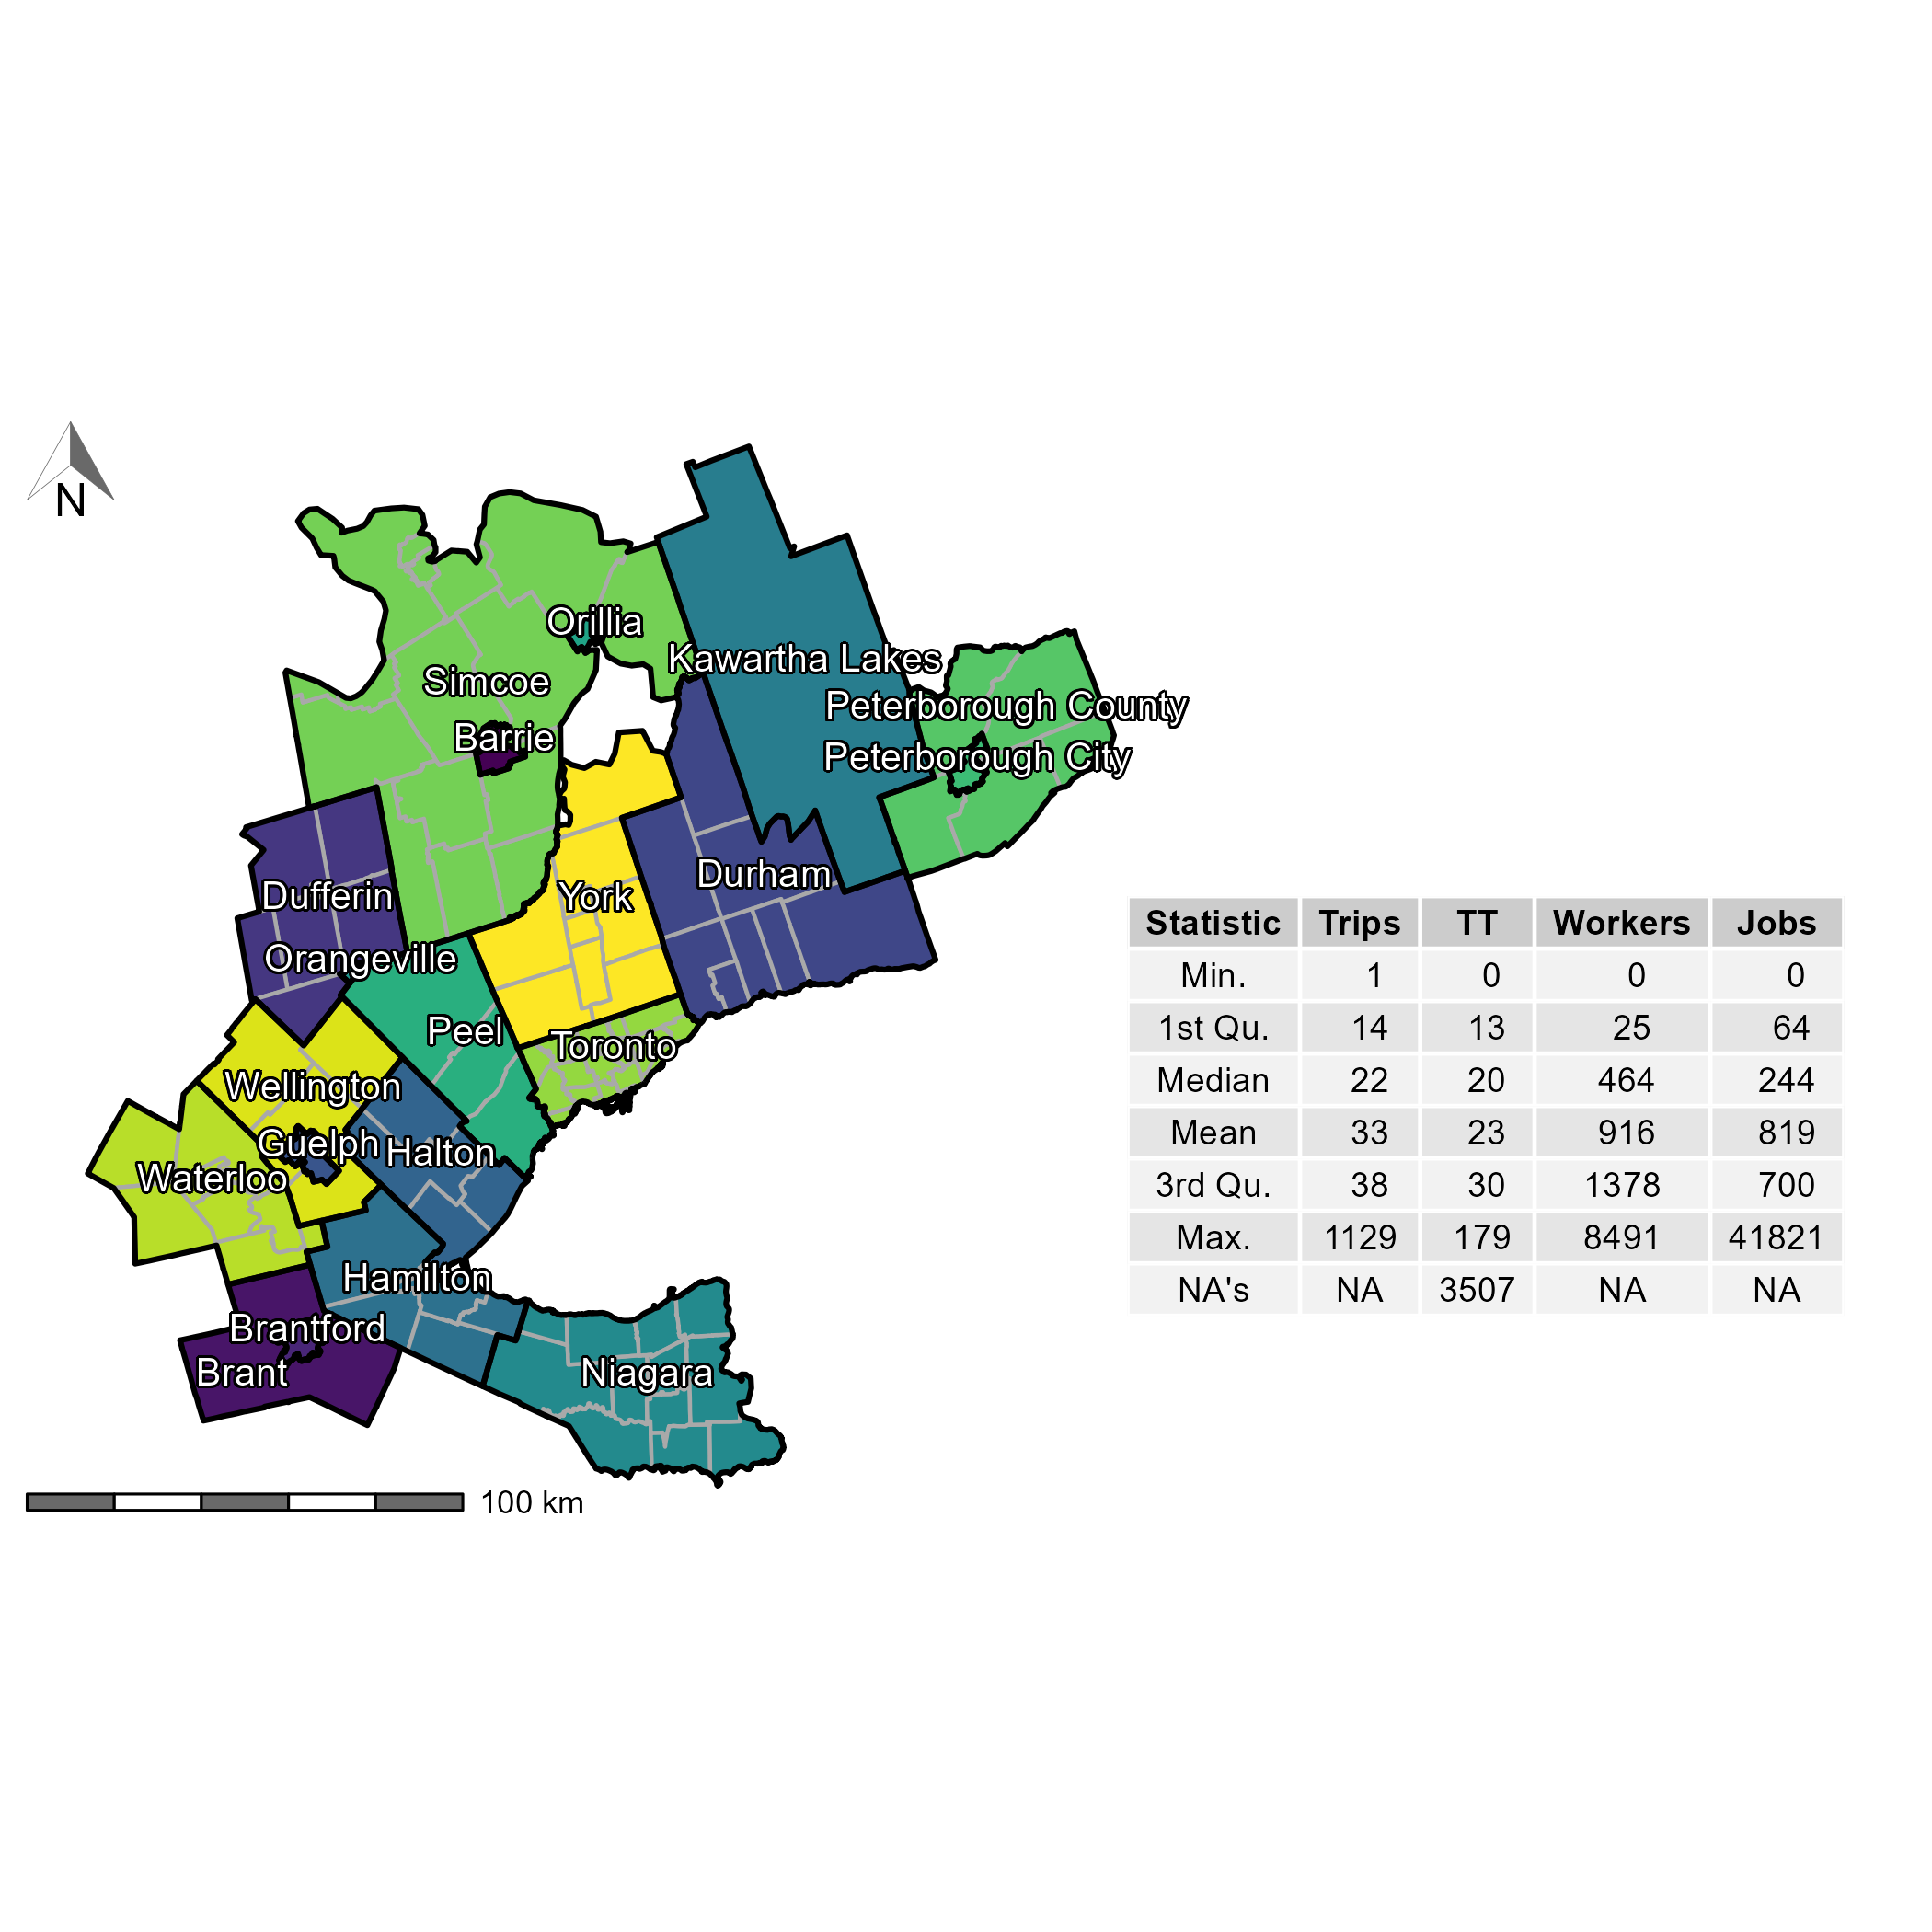
\includegraphics[width=0.8\linewidth]{images/TTS16-survey-area} 

}

\caption{\label{fig:TTS-16-survey-area}TTS 2016 study area (GGH, Ontario, Canada) along with the descriptive statistics of the trips, calculated origin-destination car travel time (TT), workers per TAZ, and jobs per TAZ. Contains 20 regions (black boundaries) and sub-regions (dark gray boundaries).}\label{fig:TTS-16-survey-area}
\end{figure}

\hypertarget{calibration-of-an-impedance-function}{%
\subsection{Calibration of an impedance
function}\label{calibration-of-an-impedance-function}}

In the synthetic example introduced in a preceding section, we used a
negative exponential function with the parameter reported by
\citet{shen1998}. For the empirical example, we calibrate an impedance
function on the trip length distribution (TLD) of commute trips.
Briefly, a TLD represents the proportion of trips that are taken at a
specific travel cost (e.g., travel time); this distribution is commonly
used to derive impedance functions in accessibility research
\citep{lopez_2017_spatial, horbachov_theoretical_2018, batista_estimation_2019}.

The empirical and theoretical TLD for this data set are represented in
the top-left panel of Figure \ref{fig:TLD-Gamma-plot}. Maximum
likelihood estimation and the Nelder-Mead method for direct optimization
available within the \{fitdistrplus\} package \citep{fitdistrplus_2015}
were used. Based on goodness-of-fit criteria and diagnostics the gamma
distribution was selected (see Figure \ref{fig:TLD-Gamma-plot}).

\begin{figure}

{\centering 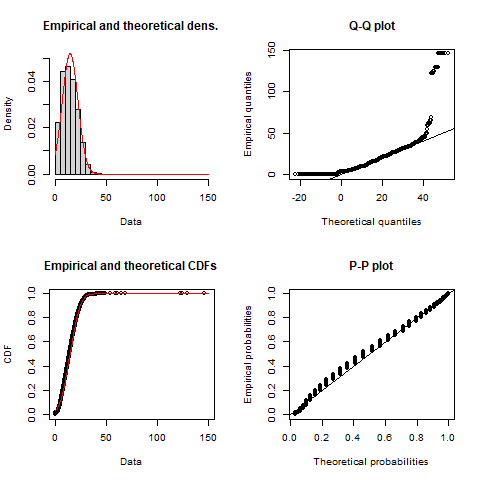
\includegraphics[width=0.8\linewidth]{images/impedance_function} 

}

\caption{\label{fig:TLD-Gamma-plot}Car trip length distribution and calibrated gamma distribution impedance function (red line) with associated Q-Q and P-P plots. Based on TTS 2016.}\label{fig:TLD-Gamma-plot}
\end{figure}

The gamma distribution is defined in Equation (\ref{gamma-dist}), where
we see that it depends on a shape parameter \(\alpha\) and a rate
parameter \(\beta\). The estimated values of these paramters are
\(\alpha=\) 2.019 and \(\beta =\) 0.094.

\begin{equation}
\label{gamma-dist}
\begin{array}{l} 
f(x, \alpha, \beta) = \frac {x^{\alpha-1}e^{-\frac{x}{\beta}}}{ \beta^{\alpha}\Gamma(\alpha)} \quad \text{for } 0 \leq x \leq \infty\\

\Gamma(\alpha) =  \int_{0}^{\infty} x^{\alpha-1}e^{-x} \,dx\\
\end{array}
\end{equation}

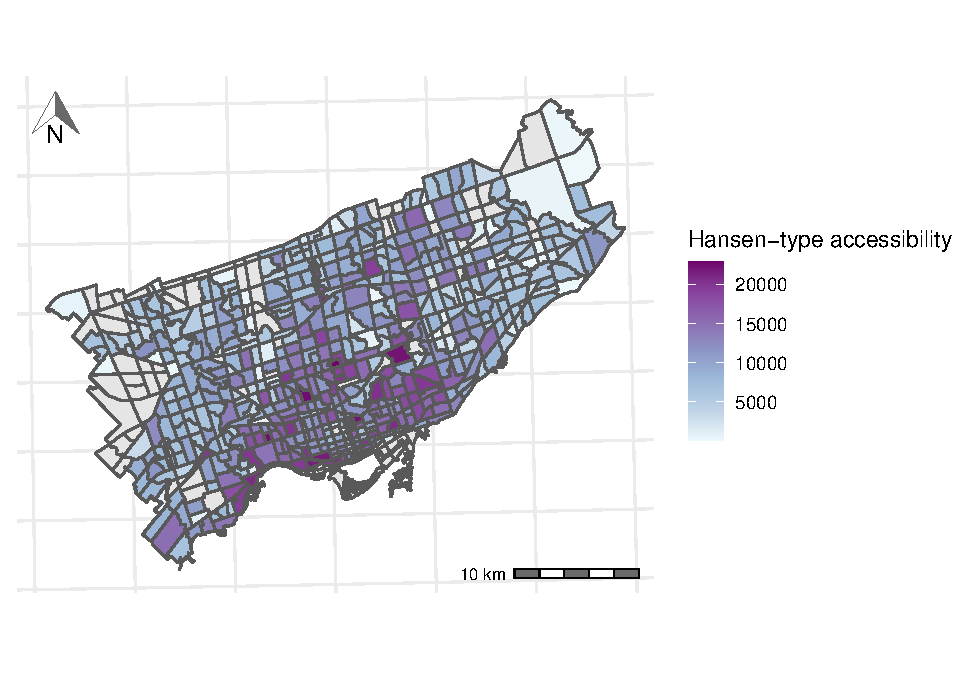
\includegraphics[width=1\linewidth]{Spatial-Availability-Refreshed_files/figure-latex/absolute-accessibility-plot-S_i-1}

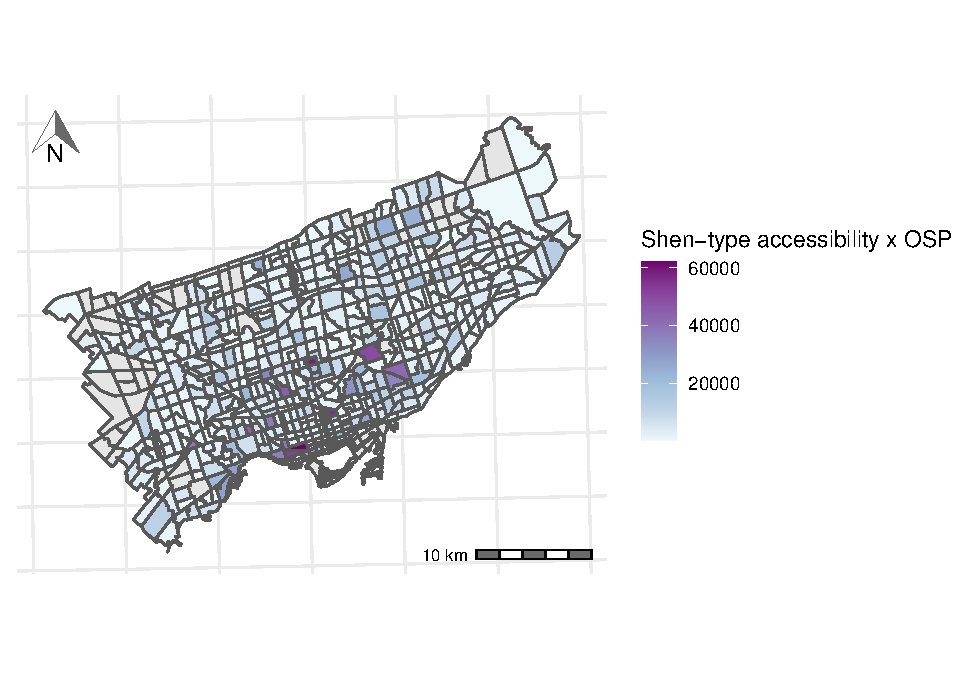
\includegraphics[width=1\linewidth]{Spatial-Availability-Refreshed_files/figure-latex/absolute-accessibility-plot-A2_i-1}

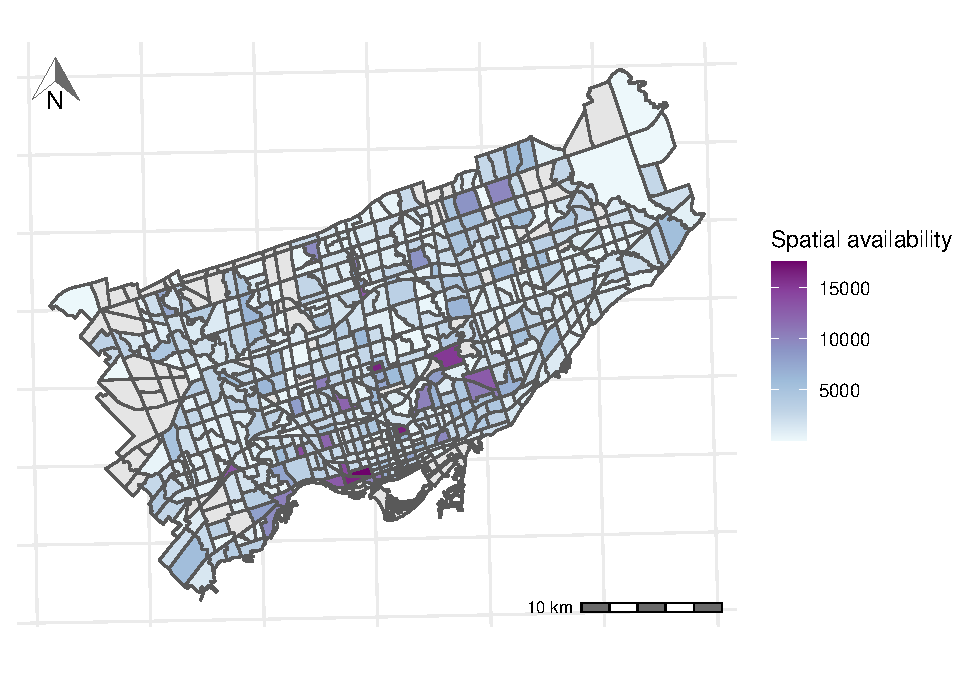
\includegraphics[width=1\linewidth]{Spatial-Availability-Refreshed_files/figure-latex/absolute-accessibility-plot-V_i-1}

\hypertarget{accessibility-and-spatial-availability-of-jobs-in-toronto}{%
\subsection{Accessibility and spatial availability of jobs in
Toronto}\label{accessibility-and-spatial-availability-of-jobs-in-toronto}}

Toronto is the largest city in the GGH and represents a significant
subset of workers and jobs in the GGH; 31\% of workers in the GGH travel
to jobs in Toronto and 40\% of jobs are located within Toronto.

\newpage

\hypertarget{discussion-and-conclusions}{%
\section{Discussion and Conclusions}\label{discussion-and-conclusions}}

Words go here.

\hypertarget{appendix-a}{%
\section{Appendix A}\label{appendix-a}}

Equivalence of Shen-type accessibility and spatial availability

Population allocation factor:

\(F^p_{ij} = \frac{P_{i\in r}^\alpha}{\sum_{i}^K P_{i\in r}^\alpha}\)

\(F^p_{A} = \frac{P_{A}^\alpha}{P_{A}^\alpha + P_{B}^\alpha + P_{C}^\alpha}\)

Cost allocation factor:

\(F^c_{ij} = \frac{f(c_{ij})}{\sum_{i=A}^K f(c_{ij})}\)

\(F^c_{A1} = \frac{f(c_{A1})}{f(c_{A1})+f(c_{B1})+f(c_{C1})}\)
\(F^c_{B1} = \frac{f(c_{A2})}{f(c_{A2})+f(c_{B2})+f(c_{C2})}\)
\(F^c_{C1} = \frac{f(c_{A3})}{f(c_{A3})+f(c_{B3})+f(c_{C3})}\)

Now let's put it together with P, and see how the denominators end up
cancelling out:

\(v_{i} = \sum_{j}\frac{O_j}{P_{i\in r}^\alpha}\frac{\frac{P_{i\in r}^\alpha}{\sum_{i}^K P_{i\in r}^\alpha} \cdot \frac{f(c_{ij})}{\sum_{i}^K f(c_{ij})}}{\sum_{i}^K \frac{P_{i\in r}^\alpha}{\sum_{i}^K P_{i\in r}^\alpha} \cdot \frac{f(c_{ij})}{\sum_{i}^K f(c_{ij})}}\)

\(v_{A} = \frac{O_1}{P_{A}^\alpha}(\frac{\frac{P_{A}^\alpha}{P_{A}^\alpha+P_{B}^\alpha+P_{C}^\alpha} \cdot \frac{f(c_{A1})}{f(c_{A1})+f(c_{B1})+f(c_{C1})}}{\frac{P_{A}^\alpha}{P_{A}^\alpha+P_{B}^\alpha+P_{C}^\alpha} \cdot \frac{f(c_{A1})}{f(c_{A1})+f(c_{B1})+f(c_{C1})} + \frac{P_{A}^\alpha}{P_{A}^\alpha+P_{B}^\alpha+P_{C}^\alpha} \cdot \frac{f(c_{B1})}{f(c_{A1})+f(c_{B1})+f(c_{C1})}+ \frac{P_{A}^\alpha}{P_{A}^\alpha+P_{B}^\alpha+P_{C}^\alpha} \cdot \frac{f(c_{C1})}{f(c_{A1})+f(c_{B1})+f(c_{C1})}}) +\)

\(\frac{O_2}{P_{A}^\alpha}(\frac{\frac{P_{A}^\alpha}{P_{A}^\alpha+P_{B}^\alpha+P_{C}^\alpha} \cdot \frac{f(c_{A2})}{f(c_{A2})+f(c_{B2})+f(c_{C2})}}{\frac{P_{A}^\alpha}{P_{A}^\alpha+P_{B}^\alpha+P_{C}^\alpha} \cdot \frac{f(c_{A2})}{f(c_{A2})+f(c_{B2})+f(c_{C2})} + \frac{P_{A}^\alpha}{P_{A}^\alpha+P_{B}^\alpha+P_{C}^\alpha} \cdot \frac{f(c_{B2})}{f(c_{A2})+f(c_{B2})+f(c_{C2})}+\frac{P_{A}^\alpha}{P_{A}^\alpha+P_{B}^\alpha+P_{C}^\alpha} \cdot \frac{f(c_{C2})}{f(c_{A2})+f(c_{B2})+f(c_{C2})}} )+\)

\(\frac{O_3}{P_{A}^\alpha}(\frac{\frac{P_{A}^\alpha}{P_{A}^\alpha+P_{B}^\alpha+P_{C}^\alpha} \cdot \frac{f(c_{A3})}{f(c_{A3})+f(c_{B3})+f(c_{C3})}}{\frac{P_{A}^\alpha}{P_{A}^\alpha+P_{B}^\alpha+P_{C}^\alpha} \cdot \frac{f(c_{A3})}{f(c_{A3})+f(c_{B3})+f(c_{C3})} + \frac{P_{A}^\alpha}{P_{A}^\alpha+P_{B}^\alpha+P_{C}^\alpha} \cdot \frac{f(c_{B3})}{f(c_{A3})+f(c_{B3})+f(c_{C3})}+\frac{P_{A}^\alpha}{P_{A}^\alpha+P_{B}^\alpha+P_{C}^\alpha} \cdot \frac{f(c_{C3})}{f(c_{A3})+f(c_{B3})+f(c_{C3})}} )\)

First, notice how the denominator on the denominator is the same across
the summation? Let's simplify it:

\(v_{A} = \frac{O_1}{P_{A}^\alpha}(\frac{\frac{P_{A}^\alpha}{P_{A}^\alpha+P_{B}^\alpha+P_{C}^\alpha} \cdot \frac{f(c_{A1})}{f(c_{A1})+f(c_{B1})+f(c_{C1})}}{\frac{P_{A}^\alpha \cdot f(c_{A1}) + P_{A}^\alpha \cdot f(c_{B1}) + P_{A}^\alpha \cdot f(c_{C1})}{(P_{A}^\alpha+P_{B}^\alpha+P_{C}^\alpha) \cdot (f(c_{A1})+f(c_{B1})+f(c_{C1}))}}) +\)
\(\frac{O_2}{P_{A}^\alpha}(\frac{\frac{P_{A}^\alpha}{P_{A}^\alpha+P_{B}^\alpha+P_{C}^\alpha} \cdot \frac{f(c_{A2})}{f(c_{A2})+f(c_{B2})+f(c_{C2})}}{\frac{P_{A}^\alpha \cdot f(c_{A2}) + P_{A}^\alpha \cdot f(c_{B2}) + P_{A}^\alpha \cdot f(c_{C2})}{(P_{A}^\alpha+P_{B}^\alpha+P_{C}^\alpha) \cdot (f(c_{A2})+f(c_{B2})+f(c_{C2}))}}) +\)
\(\frac{O_3}{P_{A}^\alpha}(\frac{\frac{P_{A}^\alpha}{P_{A}^\alpha+P_{B}^\alpha+P_{C}^\alpha} \cdot \frac{f(c_{A3})}{f(c_{A3})+f(c_{B3})+f(c_{C3})}}{\frac{P_{A}^\alpha \cdot f(c_{A3}) + P_{A}^\alpha \cdot f(c_{B3}) + P_{A}^\alpha \cdot f(c_{C3})}{(P_{A}^\alpha+P_{B}^\alpha+P_{C}^\alpha) \cdot (f(c_{A3})+f(c_{B3})+f(c_{C3}))}} )\)

See how the denominator of the denominator is the same as the
denominator of the numerator's denominator for each J (J=1, J=2, and
J=3)? Let's cancel those out and simplify:

\(v_{A} = \frac{O_1}{P_{A}^\alpha}(\frac{P_{A}^\alpha \cdot f(c_{A1})}{P_{A}^\alpha \cdot f(c_{A1}) + P_{A}^\alpha \cdot f(c_{B1}) + P_{A}^\alpha \cdot f(c_{C1})} +\)
\(\frac{O_2}{P_{A}^\alpha}\frac{P_{A}^\alpha \cdot f(c_{A2})}{P_{A}^\alpha \cdot f(c_{A2}) + P_{A}^\alpha \cdot f(c_{B2}) + P_{A}^\alpha \cdot f(c_{C2})} +\)
\(\frac{O_3}{P_{A}^\alpha}\frac{P_{A}^\alpha \cdot f(c_{A3})}{P_{A}^\alpha \cdot f(c_{A3}) + P_{A}^\alpha \cdot f(c_{B3}) + P_{A}^\alpha \cdot f(c_{C3})} )\)

Next, see how we can cancel out the \(P_{A}^\alpha\)? Let's do that.

\(v_{A} = O_1(\frac{f(c_{A1})}{P_{A}^\alpha \cdot f(c_{A1}) + P_{B}^\alpha \cdot f(c_{B1}) + P_{C}^\alpha \cdot f(c_{C1})} + O_2\frac{f(c_{A2})}{P_{A}^\alpha \cdot f(c_{A2}) + P_{B}^\alpha \cdot f(c_{B2}) + P_{C}^\alpha \cdot f(c_{C2})} + O_3\frac{f(c_{A3})}{P_{A}^\alpha \cdot f(c_{A3}) + P_{B}^\alpha \cdot f(c_{B3}) + P_{C}^\alpha \cdot f(c_{C3})} )\)

\newpage

\hypertarget{references}{%
\section*{References}\label{references}}
\addcontentsline{toc}{section}{References}

\bibliography{bibliography.bib}


\end{document}
